\documentclass[letterpaper, 12pt, oneside]{article}
% \renewcommand{\rmdefault}{phv} % Arial
% \renewcommand{\sfdefault}{phv} % Arial
\usepackage{tabu}
\usepackage{tabularx}
\usepackage{multirow}
\usepackage[none]{hyphenat} %No corte palabras
\usepackage{cite} % para contraer referencias

% idioma
\usepackage[utf8]{inputenc}
\usepackage[spanish]{babel}

% subitems enumerated
\usepackage[pointedenum]{paralist} 

%tablas
\usepackage{booktabs}

%rotar tablas
\usepackage{rotating}

%color tablas
\usepackage{colortbl}
\usepackage{comment}
\usepackage{enumitem}
\usepackage{hyperref}
\usepackage{float}	
% Image will be in the same place as you want.!!! x-/
\usepackage{subfig}
\usepackage{cite}
\hypersetup{
    colorlinks=true,
    linkcolor=blue,
    filecolor=magenta,      
    urlcolor=blue,
}

% Ecuaciones
\usepackage{mathtools}

%espaciado
\usepackage{setspace}
\onehalfspacing
\setlength{\parindent}{0pt}
\setlength{\parskip}{2.0ex plus0.5ex minus0.2ex}

%margenes según n. icontec
% \usepackage{vmargin}
% \setmarginsrb           { 4.0cm}  % left margin
%                         { 4.0cm}  % top margcm
%                         { 2.0cm}  % right margcm
%                         { 3.0cm}  % bottom margcm
%                         {   0pt}  % head height
%                         {0.0 cm}  % head sep
%                         {   9pt}  % foot height
%                         { 1.0cm}  % foot sep

\usepackage{vmargin}
\setmarginsrb           { 4.0cm}  % left margin
                        { 3.0cm}  % top margcm
                        { 2.0cm}  % right margcm
                        { 2.0cm}  % bottom margcm
                        {   0pt}  % head height
                        {0.0 cm}  % head sep
                        {   9pt}  % foot height
                        { 1.0cm}  % foot sep

% inserción url's notas de pie.
\usepackage{url}


% Paquetes de la AMS:
%Portada con título del Trabajo de Grado
\usepackage{amsmath, amsthm, amsfonts}
\addto\captionsspanish{\def\refname{\textsc{}}}

\newcommand\portada{
    \begin{titlepage}
		\begin{center}
			{\large \bf DESPLIEGUE AUTOMÁTICO DE INFRAESTRUCTURAS HPC MULTINÚCLEO Y MULTIMÁQUINA CON MÁQUINAS VIRTUALES UTILIZANDO VAGRANT }
			\vfill
  			{\large\bf AUTOR:} \\
			{\large HÉCTOR FABIO JIMÉNEZ SALDARRIAGA \par}
			\vfill
			{\large\bf UNIVERSIDAD TECNOLÓGICA DE PEREIRA} \\
			{\large\bf FACULTAD DE INGENIERÍAS} \\
			{\large\bf INGENIERÍA DE SISTEMAS Y COMPUTACIÓN} \\
			{\large\bf PEREIRA} \\
			{\large\bf 2020}
		\end{center}
	\end{titlepage}
}

\newcommand\contraportada{
\begin{titlepage}
		\begin{center}
			{\large \bf DESPLIEGUE AUTOMÁTICO DE INFRAESTRUCTURAS HPC MULTINÚCLEO Y MULTIMÁQUINA CON MÁQUINAS VIRTUALES UTILIZANDO VAGRANT }
			\vfill
			{\large\bf AUTOR:} \\
			{\large HÉCTOR FABIO JIMÉNEZ SALDARRIAGA\par}
			\vfill
			{\large\bf Documento con propuesta de proyecto de grado presentado como requisito para optar al título de Ingeniero de Sistemas y Computación\par}
			\vfill
			{\large\bf DIRECTOR:} \\
			{\large Ramiro Andrés Barrios Valencia} \\
			{\large\bf MSc. en Ingeniería de Sistemas y Computación} \\
			{\large\bf Especialista en Electrónica Digital} \\
			{\large\bf Grupo de Investigación Sirius\par}
			\vfill
			{\large\bf UNIVERSIDAD TECNOLÓGICA DE PEREIRA} \\
			{\large\bf FACULTAD DE INGENIERÍAS} \\
			{\large\bf INGENIERÍA DE SISTEMAS Y COMPUTACIÓN} \\
			{\large\bf PEREIRA} \\
			{\large\bf 2020}
		\end{center}
	\end{titlepage}
}

\sloppy
\begin{document}
\portada
\contraportada
%\contraportada
%Tabla de Contenido
	\renewcommand{\tablename}{Tabla}
	\renewcommand{\contentsname}{\centering Contenido}
	\tableofcontents
	\newpage
	\renewcommand{\listfigurename}{Lista de Figuras}
    \listoffigures
    \newpage
    \renewcommand{\listtablename}{Lista de Tablas }
    \listoftables
	\clearpage
	
	\section{Título}
	\textit{"Despliegue Automático de Infraestructuras HPC multinúcleo y multimáquina con máquinas virtuales utilizando Vagrant"}

    %Introducción al tema general
	\section{Introducción}
	
	La computación de alto rendimiento o HPC de sus siglas en inglés \textit{High Performance Computing} es un campo especial e importante de las ciencias de la computación que implica resolver problemas complejos que demandan grandes capacidades de recursos computacionales(1)(\textit{como ejemplo un gran de número de procesadores, alta cantidad de Memoria, alta capacidad de almacenamiento}), es una de las mejores maneras de computar algoritmos en diferentes campos de la ciencia como la física, medicina, bioinformática,  mecánica, química u otros problemas comunes de Big Data. Estas tareas y procesos son  grandes para ser realizados en una sola máquina, por ello se hace necesario construir lo que se denomina un \textit{Clúster} de computadores definido como un grupo de múltiples nodos o computadores que trabajan de manera conjunta y distribuida para cumplir con una meta. 
	
	Debido a la naturaleza de múltiples computadores conectados entre sí, existen diferentes modelos de computación paralela y distribuida que han sido desarrollados e implementados por la comunidad científica para la coordinación de los computadores pertenecientes a un Clúster, de manera que su uso sea eficiente y efectivo. Un modelo muy utilizado y popular es el \textit{paso de mensajes}, una técnica empleada en programación concurrente para aportar sincronización entre procesos y permitir la exclusión mutua; su diseño esta pensando para algoritmos y programas que exploten la existencia de múltiples procesadores en un Clúster. MPI es el estándar de facto preferido por la comunidad HPC a la hora de realizar implementaciones de paso de mensajes.

    Tradicionalmente, configurar un clúster de computadores, por ejemplo, un clúster MPI, es una tarea desafiante que requiere que estudiantes, aficionados, novatos y avanzados pasen un tiempo configurando los diferentes elementos del sistema operativo, configuraciones de red, configuraciones de aplicaciones terceras. Sin embargo, en los últimos años el avance del Cloud Computing y la implementación de metodologías ágiles que impulsan culturas como la DevOps han hecho que la automatización en todas las etapas sea masiva  \cite{devopsH2} \cite{devopsH3} , gracias a esto  diferentes proyectos de software libre y de código abierto han visto la luz, como \strong{Vagrant}, una herramienta de código abierto que permite la creación y configuración de ambientes virtuales portables y ligeros. En este proyecto se presenta una implementación utilizando Vagrant para realizar  la construcción automática de un clúster MPI multinúcleo y multimáquina.
    
    %Formulación del problema o descripción del mismo.
    \section{Formulación del Problema}
    
    La infraestructura como código o IaC (Infraestructure as Code) es uno de los pilares fundamentales de la cultura DevOps, la IaC hace referencia a la práctica de poder administrar, aprovisionar, actualizar, monitorear y configurar la infraestructura TI de las empresas, utilizando scripts en diferentes lenguajes de programación en lugar de configurar las máquinas de manera manual\cite{devopsH4} \cite{iac}. La IaC trata todas las configuraciones de la infraestructura TI como código, permite a las máquinas virtuales gestionarse de manera programada y automática, lo que elimina la necesidad de realizar configuraciones manuales por parte del personal a cargo de componentes individuales de hardware. Esto hace que la infraestructura sea muy moldeable, es decir, escalable y replicable siendo agnóstico al hardware y al proveedor de servidor cloud, además se utilizan las mismas prácticas implementadas para la gestión y versionamiento del código de aplicaciones de software. 

    La implementación y construcción de un clúster MPI implica  tiempo y conocimiento de todos los elementos que lo componen, es necesario conocer un completo detalle de como realizar la instalación de cada uno de los componentes del clúster, algunas tareas que son repetitivas se puede automatizar implementando IaC; ejemplo de ello es la creación de usuarios con sus niveles de privilegios, las configuraciones de seguridad, la configuración de servicios, las configuraciones de sistemas de archivos compartidos, entre otras tareas repetitivas. Es necesario en un clúster MPI asegurar la inmutabilidad y homogeneidad en las configuraciones realizadas en los nodos que lo componen.\cite{repositoriounal}
    \clearpage
    
    %Justificación del trabajo de grado 
    \section{Justificación}
    En la universidad Tecnológica de Pereira, el programa de Ingeniería de Sistemas y Computación brinda la posibilidad a los estudiantes de pregrado tomar como materia electiva de noveno semestre Computación de Alto Desempeño(\textit{CAD}) o HPC(\textit{High Performance Computing}), en esta materia el estudiante tiene la posibilidad de aprender y conocer todos los elementos que implica la computación de alto desempeño, además el aprendizaje a tratar grandes volúmenes de datos, ejecutar grandes y complejos cálculos científicos, en tiempos aceptables, medibles, con una precisión adecuada a los diferentes problemas establecidos por el docente. Los estudiantes también aprenden a construir un mini clúster replica con nodo maestro y múltiples nodos esclavos, esta simulación permite que el estudiante se haga a una idea de las diferentes arquitecturas paralelas y distribuidas encontradas en un clúster real, así como los diferentes modelos de memoria. La construcción y montaje de este es realizada por los estudiantes con la guía del docente. 
    
    Durante el segundo semestre del año 2018 en el curso de Computación de Alto Desempeño, se tuvo la oportunidad de construir el clúster: el montaje, aprovisionamiento y puesta en marcha. Durante las múltiples revisiones se observaba que se presentaban algunas fallas como : 
    
    \begin{itemize}
        \item Falta de configuraciones de networking en las máquinas esclavas.
        \item Falta de idempotencia y definiciones específicas para las configuraciones de las máquinas virtuales.
        \item Fallos de arranque con las máquinas virtuales.
        \item Pérdida de estados de las máquinas esclavas.
    \end{itemize}
    
    Es así como los puntos anteriores generaron cuestionamientos y reflexiones acerca de la forma de automatizar el proceso de la construcción del clúster de HPC utilizando tendencias modernas como IaC (\textit{Infrastructure as Code}) e implementación de herramientas de la cultura DevOps como \textbf{Vagrant} y \textbf{Git}. 
    En  este  proyecto  se  presenta  una  implementación que automatiza la construcción automática de un clúster MPI multinúcleo y multimáquina, de esta manera el estudiante podrá poner su atención principalmente en los conceptos de modelos de algoritmos concurrentes, paradigmas y modelos de la programación paralela e implementación de la programación de memoria distribuida y paso de mensajes con MPI. 
    
    %Objetivos 
	\section{Objetivos}
	
	\subsection{Objetivo general}
	
	Diseñar e implementar un conjunto de programas para el aprovisionamiento automático de un clúster computacional sobre máquinas virtuales, que soporten procesos con MPI
	
	\subsection{Objetivos específicos}
	\begin{itemize}
    	\item Obtener la lista de requerimientos, limitaciones, especificaciones para el diseño del aprovisionamiento automático utilizando Vagrant.
    	\item Desarrollar e implementar un sistema de archivos distribuido en el Clúster MPI.
        \item Realizar pruebas de ejecución y funcionamiento del clúster.
        \item Realizar pruebas de ejecución y desempeño multimáquina en el Clúster MPI compuesto por máquinas virtuales.
    \end{itemize}

    \section{Marco Referencial}
    \subsection{Marco Histórico}
    
    
    La historia de la computación de alto desempeño tiene su orígen en los conceptos informáticos que se remontan a 2400 a. C. con la creación del ábaco.
    La informática electrónica comenzó a mediados de la década de 1940 con la ENIAC, la primera computadora electrónica de uso general \cite{hpcHistory}.
    
   << La primera asociación de High-Performance Computing (HPC) comenzó en 1985 cuando la National Science Foundation estableció una asociación entre cinco centros de investigación: San Diego Supercomputer Center (SDSC) en la Universidad de California en San Diego, Pittsburgh Supercomputer Center (PSC) en la Universidad de Pittsburgh, el Centro Nacional de Aplicaciones de Supercomputación (NCSA) en la Universidad de Illinois Champagne-Urbana, el Centro de Teoría Cornell en la Universidad de Cornell y el Centro John von Neumann en la Universidad de Princeton.
    
    En 1997, la NSF anunció dos nuevas asociaciones de supercomputación, la Asociación Nacional para la Infraestructura Computacional Avanzada (NPACI) y la Alianza Nacional de Ciencia Computacional (NCSA). La financiación de estas asociaciones se limitó a cinco años.
    
    La siguiente iteración de las asociaciones de HPC fue TeraGrid, establecida en 2001. La financiación de TeraGrid también se limitó a cinco años. Se proporcionó una extensión de sexto año para cerrar la brecha entre TeraGrid y la asociación XSEDE, que recibió fondos en 2011. La financiación fue por cinco años, hasta 2016, momento en el que se estableció XSEDE 2>> \cite{hpcHistory} .
    
    En cuanto a la cultura DevOps, se considera a Andrew Clay su creador, junto con el belga Patrick Debois. Ambos empezaron a trabajar en 2008 para llevar la filosofía Agile al mundo de la administración de sistemas. El resultado de su trabajo se haría público en San José (California) en 2009 y un año más tarde en Europa \cite{devopsHistory1}  .
    
    \subsection{Marco Conceptual}
    
    A continuación se describen los conceptos fundamentales para el entendimiento del presente proyecto
    
    \begin{itemize}
    
       
        
        \item \textit{Gestor de Paquetes:} Un gestor de paquetes es una pieza de software que permite instalar, obtener, eliminar, actualizar software y sus dependencia en un sistema operativo, como se menciona en \cite{packagemanager}, la idea principal de esto es tener un control total de las librerías y dependencias que son requeridas por un software; mediante la implementación de una heurística se tiene una traza de todos las librerías instaladas en el sistema de archivos. El sistema gestor de paquetes logra esto gracias a la construcción de un árbol de dependencias, que se encuentra definido en un archivo de configuración dentro de los paquetes(\textit{por ejemplo RedHat, tiene un sistema de empaquetamiento, las extensiones \textbf{rpm}, debian con los archivos \textbf{deb}}), estos contienen una definición exacta de las ubicaciones donde se instalarán las dependencias según el estándar lsb de las distribuciones Linux, además de detectar todos los conflictos posibles mediante SAT solvers \cite{packagemanager}.
        
        \item \textit{Multithreading:} 
        En arquitectura de computadores, Multithreading o multihilo es la habilidad de una CPU (Unidad Central de Procesamiento) o de un core en un procesador multi-core, de proveer múltiples hilos de ejecución concurrentes, siendo esto soportado por el sistema operativo. En un sistema multihilo, los hilos comparten los recursos de un solo core o de múltiples cores, lo que incluye las unidades de computación, las caches de CPU y el TLB (Translation Lookaside Buffer)\cite{Multithreading2}.
        El multithreading busca incrementar el uso de un solo core mediante la utilización, tanto de paralelismo a nivel de hilo, como de paralelismo a nivel de instrucción\cite{Multithreading1}.


        \item \textit{Multiproceso:} El Multiprocesamiento o multiproceso es el uso de dos o más procesadores (CPU) en una computadora para la ejecución de uno o varios procesos de manera concurrente. Las ventajas principales son: el incremento del rendimiento, ya que al incrementarse el número de procesadores, se puede realizar mayor cantidad de trabajo en un menor tiempo; más económico al escalarse, al compararse con sistemas de monoprocesamiento, ya que es posible compartir periféricos, almacenamiento, suministro de energía...; y mayor fiabilidad, ya que al tener más de un procesador las funciones pueden ser distribuidas, y en el caso de que ocurra un fallo en un procesador, el sistema no se detiene sino que lo hace más lento \cite{Multiprocesamiento}. 
        
        \item \textit{Control de versiónes:} Es un componente de la administración de configuraciones de software, también es conocido como control de revisiones, control de código fuente, o administración de código fuente. Se define como la gestión de cambios que se realiza de diferentes elementos o configuraciones en productos de software y sistemas informáticos.Gracias a esta necesidad surgieron los sistemas de control de versiónes. Entre ellos se puede encontrar : 
        
        \begin{itemize}
            \item Git 
            \item Subversión 
            \item Mercurial
        \end{itemize}
        
        \item \textit{Git:} Git es un sistema de control de versiones distribuido, creado por Linus Torvalds el 7 de abril de 2005 para poder mejorar el flujo de trabajo de los desarrolladores del kernel de Linux, basado en algunas ideas de Bitkeeper. Su desarrollo fue potenciado por la comunidad debido al rompimiento comercial de Bitkeeper como compañía, su primera puesta en escena fue el manejo de cambios del código fuente del kernel Linux que cuenta con cientos y miles de desarrolladores alrededor de todo el mundo. En la actualidad es el control de versión distribuido mas utilizado y es una de las herramientas mas necesarias para cualquier desarrollador de software. 
        
        \item \textit{DevOps:} Developer Operations, una palabra que inicialmente surgió de una discusión entre Andrew Clay y Patrick Debois en el año 2008. Ambos desarrolladores experimentados les preocupaban los inconvenientes de la metodología ágil y querían encontrar algo mejor. La idea comenzó a extenderse lentamente después de realizar un evento DevOpsDays celebrado en Bélgica en 2009, la palabra se convirtió en una palabra de moda. 
        
        DevOps es una idea, que busca la combinación de filosofías, prácticas y herramientas culturales que aumenta la capacidad de una organización para entregar aplicaciones y servicios con gran valor,  evolucionando y mejorando productos a un ritmo más rápido que las organizaciones que usan procesos tradicionales de desarrollo de software y gestión de infraestructura. Esta velocidad permite a las organizaciones servir mejor a sus clientes y competir de manera más efectiva en el mercado.\cite{devops2}
        
        La implementación de una cultura DevOps garantiza que los desarrolladores ahora puedan participar en los despliegues de aplicaciones a producción, los administradores pueden escribir scripts y los ingenieros de QA saben cómo resolver otros problemas además de las pruebas. Los procesos pueden automatizarse y nadie tiene que esperar, ya que ahora pueden trabajar más estrechamente y encontrar soluciones más rápidas y mejores. Esto permite que haya una mejor comunicación y comprensión entre los equipos de desarrollo y operaciones. \cite{devops}
        
        
        \item \textit{Metodologías Ágiles:} 
        Son aquellas metodologías que permiten adaptar la forma de trabajo a las condiciones del proyecto, consiguiendo una respuesta flexible e inmediata ante las necesidades del desarrollo del proyecto y las circunstancias específicas del entorno \cite{agiles}.
        Estas metodologías son especialmente útiles cuando se tiene que abordar un proyecto donde probablemente ocurrirán cambios, ya que proporcionan mecanismos para afrontar estos cambios manteniendo el máximo valor para el cliente, incrementando así la probabilidad de finalizar con éxito el proyecto \cite{agiles2} \cite{agiles3}.
        
    \end{itemize}
    
    \subsection{Marco Teórico}
    
    
    \begin{itemize}
         \item \textit{Hypervisor:}Un hypervisor, conocido también como monitor de máquina virtual (\textit{Virtual Machine Manager}), es un software que crea y ejecuta máquinas virtuales (VMs) y que, además, aísla el sistema operativo y los recursos del hypervisor de las máquinas virtuales. El rol importante de este herramienta es permitir realizar todas las actividades de administración y gestión de las máquinas virtuales.\cite{hypervisor}
        
        \item \textit{máquina Virtual:} Una máquina virtual (VM  del ingles Virtual Machine) es un entorno virtual que funciona como sistema informático virtual con su propia CPU, memoria, interfaz de red y almacenamiento, pero se crea en un sistema de hardware físico, en el que está instalado un hypervisor libre o comercial al que se llama "host", y las VMs que utilizan sus recursos se llaman "guests".  Las VMs se encuentran aisladas del resto del sistema, pero puede haber varias VMs en una sola pieza de hardware, como un servidor.\cite{virtualmachine}
        
        \item \textit{Message Passage Interface:} Es el estándar que define la sintaxis, la semántica y demás elementos de la especificación MPI para  una interfaz común de funciones implementadas para el paso de mensajes. 
        En la actualidad MPI cuenta con una conjunto de funciones convergentes en una librería. El estándar MPI es construido a través de un proceso abierto y comunitario alrededor de todo el mundo, conformada por investigadores, científicos, desarrolladores de aplicaciones y múltiples vendedores que trabajan en problemas de computación de alto desempeño y paradigmas de procesamiento paralelo. Este estándar busca explotar el uso de la programación paralela y el paso de mensajes entre procesos, posibilitando utilizar todos los cores existentes en un procesador o en máquinas multiprocesador.
        Según el MPI-2019-Draft-report\cite{MpiDraf} [2] MPI no es un lenguaje de programación en sí, y todas las operaciones MPI son expresadas como funciones, subrutinas o métodos, que definen de manera clara todos los mecanismos para un estándar de paso de mensajes.  
        
        
        \item \textit{Network File System:} 
        El sistema de archivos en red (Network File System, NFS) es una implementación cliente/servidor que permite a un usuario de un equipo ver, almacenar y actualizar archivos en un equipo remoto como si se estuviera en el equipo del usuario. Este protocolo es uno de varios estándares de sistemas de archivos distribuidos mas implementado en dispositivos de almacenamiento (NAS).
        El protocolo NFS permite al usuario o administrador del sistema designar como accesible todo o una porción del sistema de archivos en un servidor. Esta parte puede ser accedida por los clientes con los privilegios que se asignen a cada archivo, sólo de lectura o lectura y escritura. NFS utiliza llamadas de procedimiento remoto (RPC) para enrutar solicitudes entre clientes y servidores\cite{NFS}.
        Todos los sistemas Unix pueden trabajar con este protocolo; si se involucran sistemas Windows, se debe utilizar Samba en su lugar\cite{NFS2} 
    \end{itemize}
  

    %Delimitación
    \section{Alcance}
    
    Este proyecto tiene como fin realizar la implementación de scripts que permitan automatizar la creación de un clúster HPC que permita realizar la ejecución de aplicaciones y algoritmos desarrollados utilizando MPI mediante el uso de máquinas virtuales automatizadas utilizando la herramienta Open Source \textbf{Vagrant},  una herramienta de línea de comandos  que permite administrar el ciclo de vida de máquinas virtuales de manera consistente y maximizar la productividad soportando múltiples hypervisores como VirtualBox, VMware, AWS, entre otros.
    
    Pensando en futuras implementaciones, se tiene la posibilidad de que a partir de los resultados que se obtuvieron en el presente proyecto, se podría implementar una configuración para otros proveedores de la nube como AWS o Google Cloud Platform. 
    \section{Diseño Metodológico}
     \begin{itemize}
        \item 

  El enfoque y método seguido para la ejecución de este proyecto es \textit{“aprender haciéndolo”}, parte desde el aprendizaje de las características de Vagrant y la programación de los scripts en Ruby hasta la parametrización y configuración de cada una de las tecnologías y software implicados para dejar el clúster de MPI funcionando, todo ello llevado a cabo desde un punto de vista práctico.

  
        \item Tipo de investigación
        
        Basados en los puntos anteriores se considera que éste es un Proyecto de aplicación ya que se pretende desarrollar e implementar la automatización del clúster, buscando resolver problemas de la vida cotidiana y controlar situaciones prácticas, permitiendo la obtención de nuevos conocimientos por medio de la investigación realizada y la generación de un entregable después de la culminación de dicha investigación. 
    
        En esta investigación se utilizará un enfoque cualitativo, además, se empleará el método científico.
        
        \item Estrategias
        
        Se llevará a cabo un conjunto de pruebas sobre el sistema, para establecer si cumple con las estimaciones del proyecto y si es funcional.
     \end{itemize}
    \newpage
    \subsection{Metodología}
    \textbf{Fases de la Metodología}
    \begin{itemize}
        \item Fase 1 : Recolección de requerimientos y análisis de la información
        \item Fase 2 : Diseño e implementación de despliegues automáticos
        \item Fase 3 : Documentación y conclusiones
    \end{itemize}\\
       \clearpage
    
    \section{Implementación}
    \subsection{Configuraciones Iniciales y Prerrequisitos}
    Para realizar este proyecto de grado, las instalaciones de pruebas se implementaron utilizando el sistema operativo Windows 10 Professional, junto con la herramienta de Windows Subsystem for Linux (WSL2).
    
    El computador portátil utilizado para hacer el desarrollo de este trabajo de grado tiene las siguientes características : 
    \begin{itemize}
        \item Marca : Lenovo
        \item Referencia : Thinkpad X1 6th
        \item Procesador : Intel(R) Core(TM) i7-8650U CPU @1.90GHz 2.11GHz 
        \item Memoria Ram : 16GB
        \item Disco Duro : 1TB SSD 
        \item Sistema Operativo : Windows 10 Professional, Build 19631.mn\_release200514
    \end{itemize}
    
    A continuación se detallarán los elementos que deben ser instalados para poder llevar acabo todo el proyecto, además de algunos detalles de la implementación y apuntes sobre las herramientas.
    
    \subsubsection{Instalación de Oracle VM VirtualBox}
    VirtualBox es un Hypervisor opensource para procesadores Intel/AMD multiplataforma; al momento de realizar este documento la versión estable es la \textbf{6.1.6}. Su instalación se realiza mediante un wizard de manera guiada, éste instala los elementos necesarios para poder realizar la virtualización de todos los dispositivos necesarios por las máquinas virtuales, además de instalar drivers adicionales para montar pseudo dispositivos de red como se muestra en las siguientes imágenes. 
    Actualmente existe la versión privativa Oracle VM VirtualBox, que es gratuita únicamente \textbf{bajo uso personal o de evaluación} como es el de este proyecto\footnote{(VirtualBox Personal Use and Evaluation License o PUEL)}.Oracle Corporation adquirió Sun Microsystems en enero de 2010, es por esto que hubo un cambio de la marca del producto a \textit{Oracle VM VirtualBox}\cite{oracle}.
    
    Es necesario ingresar al sitio web de VirtualBox y realizar la descarga del instalador.
    \begin{center}
    \begin{figure}[H]
        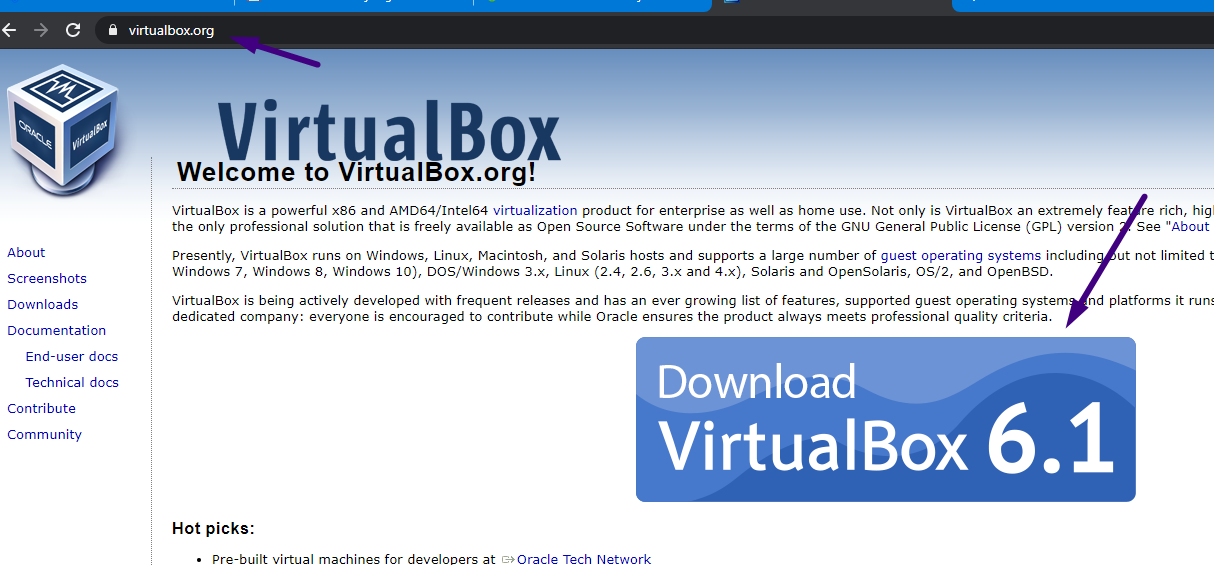
\includegraphics[scale=1]{img/install/virtualbox1.png}
        \caption{Sitio Web Oficial, https://www.virtualbox.org/ .}
        \label{fig:vbox1}
    \end{figure}
    \end{center}

    Una vez terminada la descarga, es necesario realizar la validación de que fue correctamente descargado, esto se puede validar con una firma hash. 
    \begin{center}
     \begin{figure}[H]
        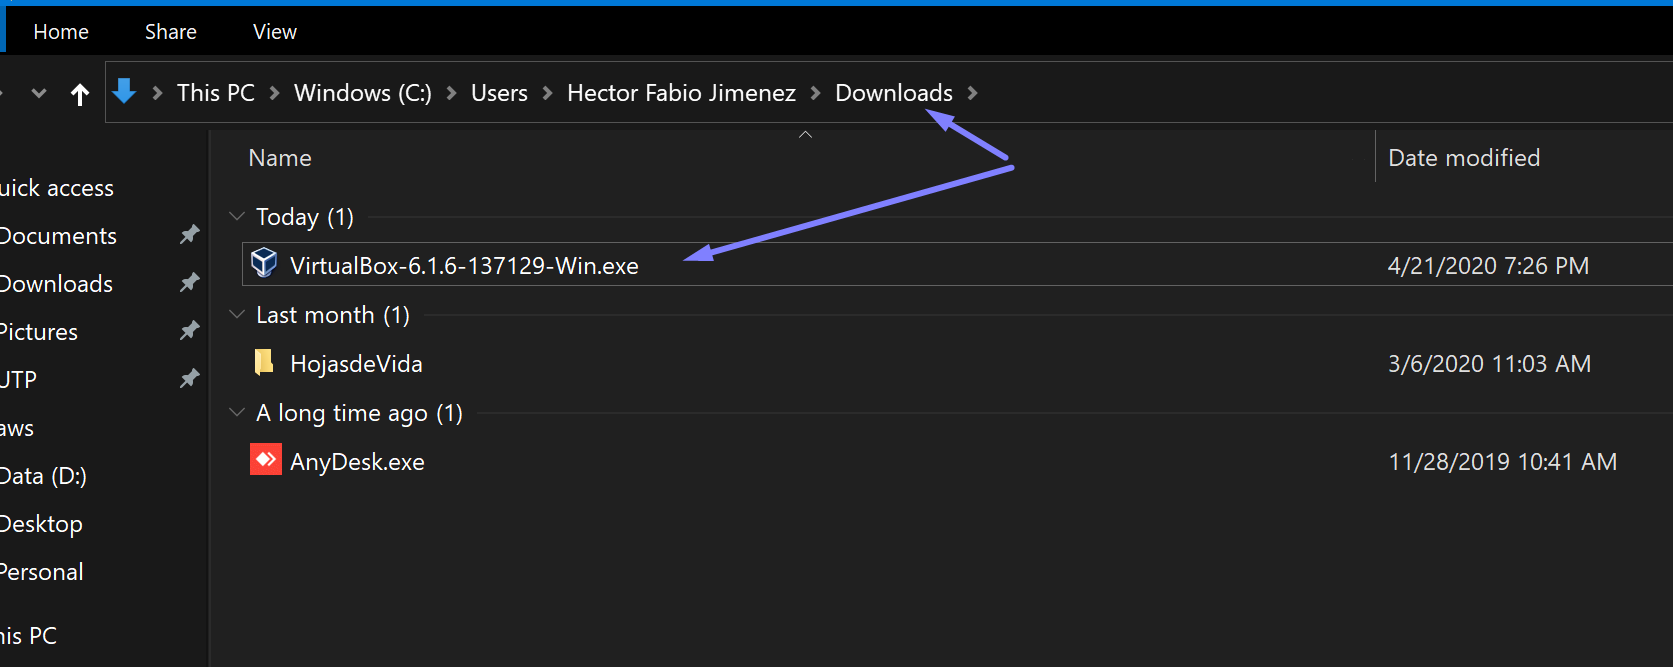
\includegraphics[scale=0.7]{img/install/virtualbox2.png}
        \caption{Instalador Virtualbox, Versión \textbf{6.1.6}.}
        \label{fig:vbox2}
    \end{figure}       
    \end{center}

    Para proceder con esto, se ejecuta el instalador como administrador y se continua con las instrucciones del setup wizard, como se muestra en la Figura.\ref{fig:vbox3}.
    \begin{center}
    \begin{figure}[H]
        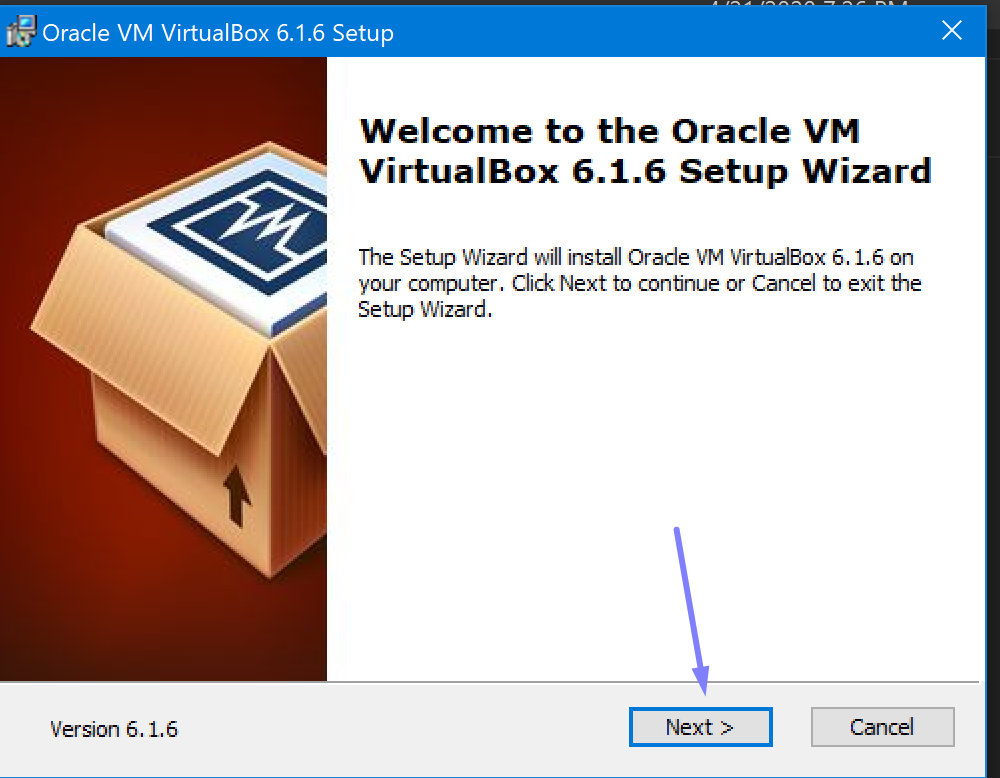
\includegraphics[scale=0.8]{img/install/virtualbox3.png}
        \caption{Ejecución de Wizard como administrador.}
        \label{fig:vbox3}
    \end{figure}    
    \end{center}
    
    \begin{center}
    \begin{figure}[H]
        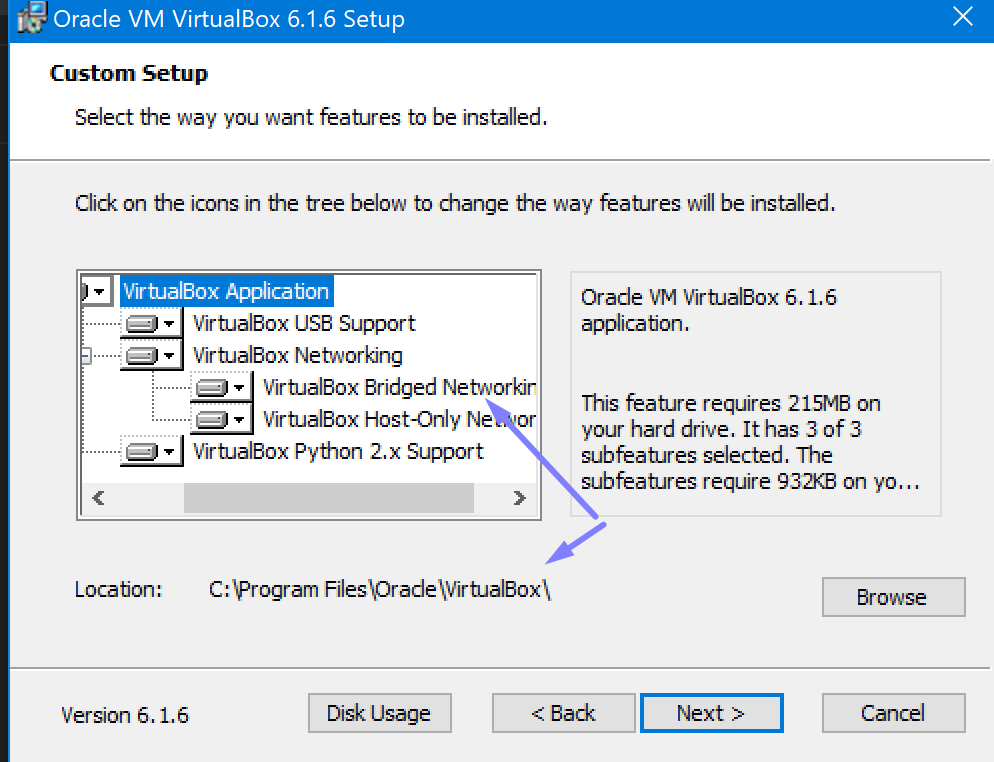
\includegraphics[scale=1]{img/install/virtualbox4.png}
        \caption{Es obligatorio instalar VirtualBox con las opciones resaltadas, soportando los dos modos de Interfaz de red.}
        \label{fig:vbox4}
    \end{figure}  

        \begin{figure}[H]
            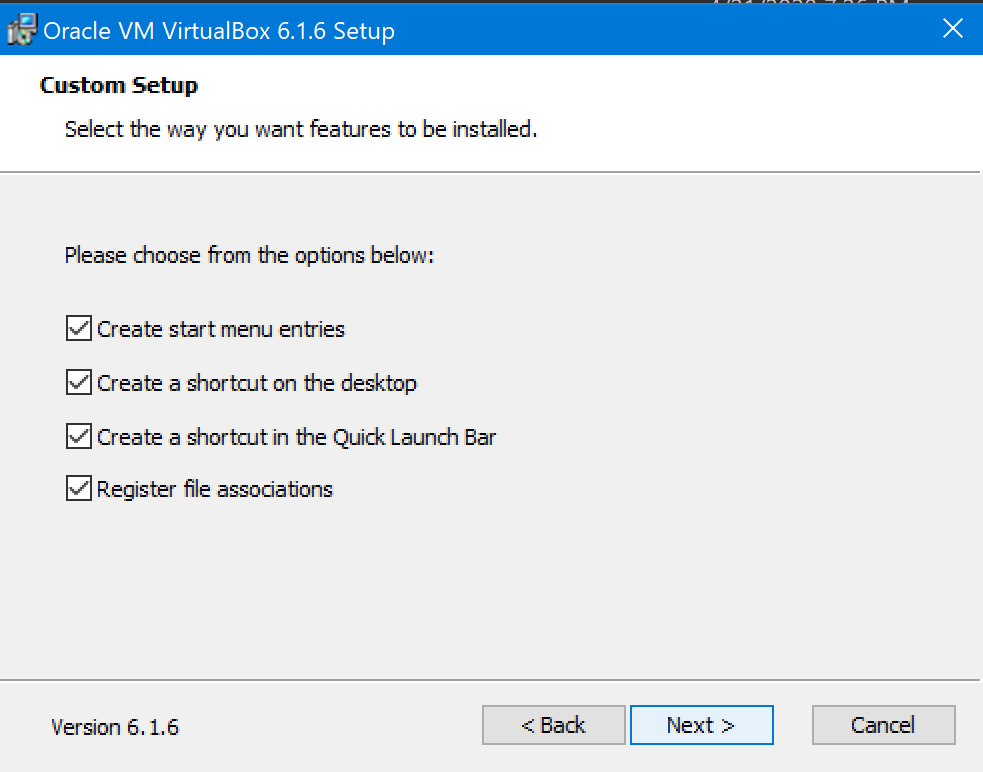
\includegraphics[scale=1]{img/install/virtualbox5.png}
            \caption{Se permite crear accesos directos y registro de extensiones preferencia, Wizard.}
            \label{fig:vbox5}
        \end{figure}
        
        \begin{figure}[H]
            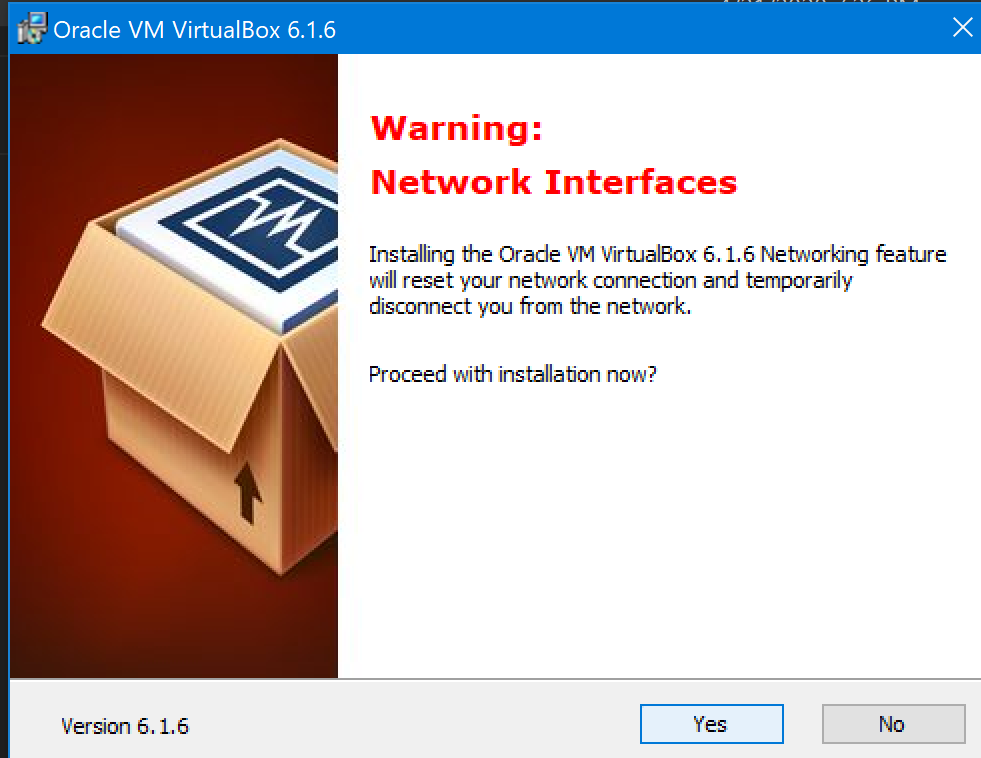
\includegraphics[scale=1]{img/install/virtualbox6.png}
            \caption{Características de Networking  y Driver requieren reinicio de la máquina host.}
            \label{fig:vbox6}
        \end{figure}
     \end{center}  
    De esta manera el sistema operativo ya debería contar con el hypervisor VirtualBox instalado. Una buena práctica es posteriormente ejecutar VirtualBox para validar que no existan problemas de dependencias o falta de librerías \textit{DLL} en el sistema operativo. Se debe observar algo como en la Figura.\ref{fig:vbox7}
    \begin{center}
    \begin{figure}[H]
        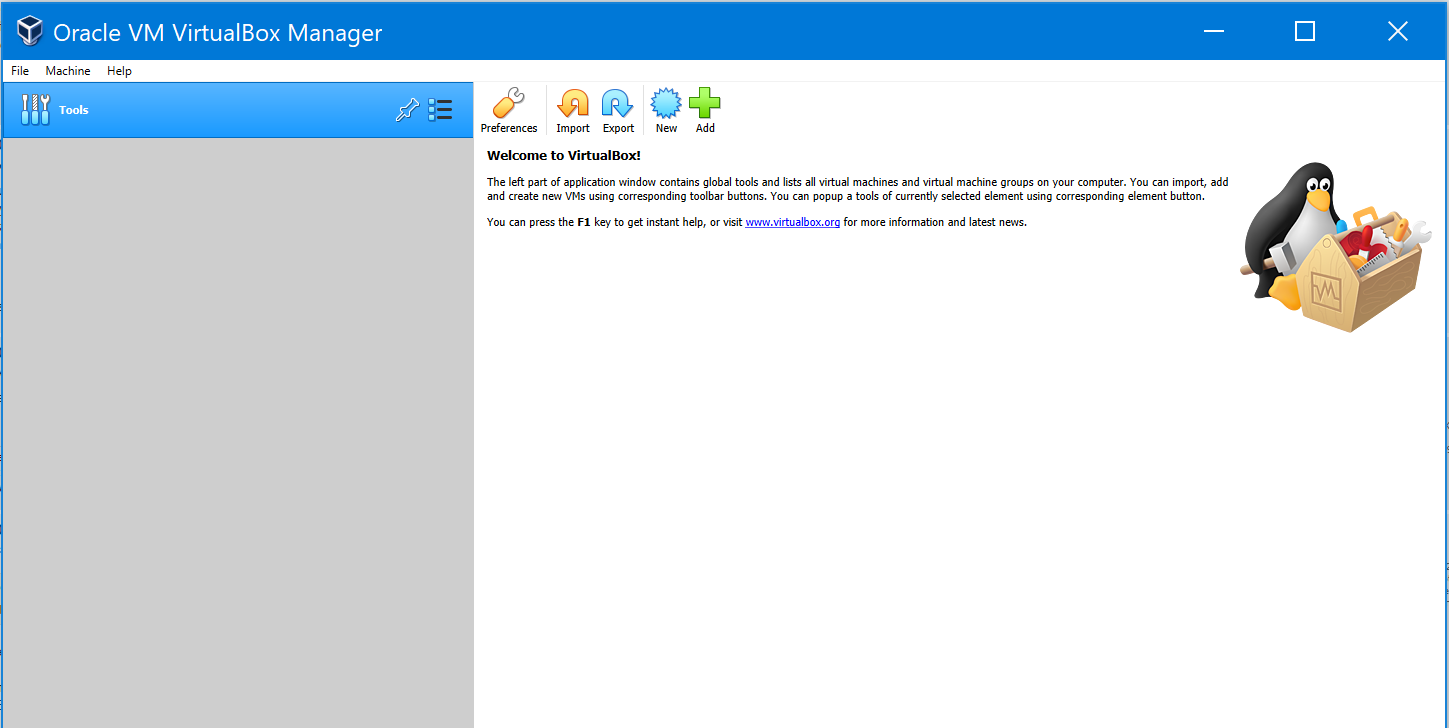
\includegraphics[scale=0.7]{img/install/virtualbox7.png}
        \caption{Instalación completa VirtualBox.}
        \label{fig:vbox7}
    \end{figure}
    \end{center}
    
    \subsubsection{Instalación de Vagrant}
    Vagrant como se ha mencionado previamente es una herramienta de código abierto disponible para Windows, MacOS X,  GNU/Linux que permite la creación y configuración de ambientes virtuales portables, repetibles y ligeros, de manera programática. Mediante scripts desarrollados en el lenguaje de programación Ruby se puede definir las características de las máquinas virtuales, entre ellas la cantidad de memoria ram, cantidad de CPUs virtuales, todas las configuraciones de red, además de tener funciones adicionales mediante algo que se conoce como "provisioners" que permite instalar software, alterar configuraciones y mucho más como parte del proceso de creación e inicialización.\footnote{Esto sucede al momento de realizar la ejecución del comando \textbf{\texttt{vagrant up}}. }
    
    Esta herramienta, utilizada para construir máquinas virtuales preconfiguradas\footnote{La preconfiguración hace referencia al uso de la imagen de un sistema operativo base, éstas pueden ser encontradas en \url{https://app.vagrantup.com/boxes/search}. También puede ser un término usado para referirse a la preinstalación de software.  },  fue desarrollada por Mitchell Hashimoto en el año 2010, junto a su compañero de trabajo John Bender, ambos fundarían la compañía que hoy brinda el soporte comercial \textbf{HashiCorp Inc}, actualmente con una gran variedad de productos orientados a la cultura DevOps\footnote{otra gran herramienta de esta compañia es packer, \url{https://www.packer.io/}}. La forma mas fácil de obtener Vagrant instalado y corriendo, según el libro oficial \cite{vagrantup}, es descargar el software del sitio web \textbf{www.vagrantup.com}
     
    \begin{figure}[H]
        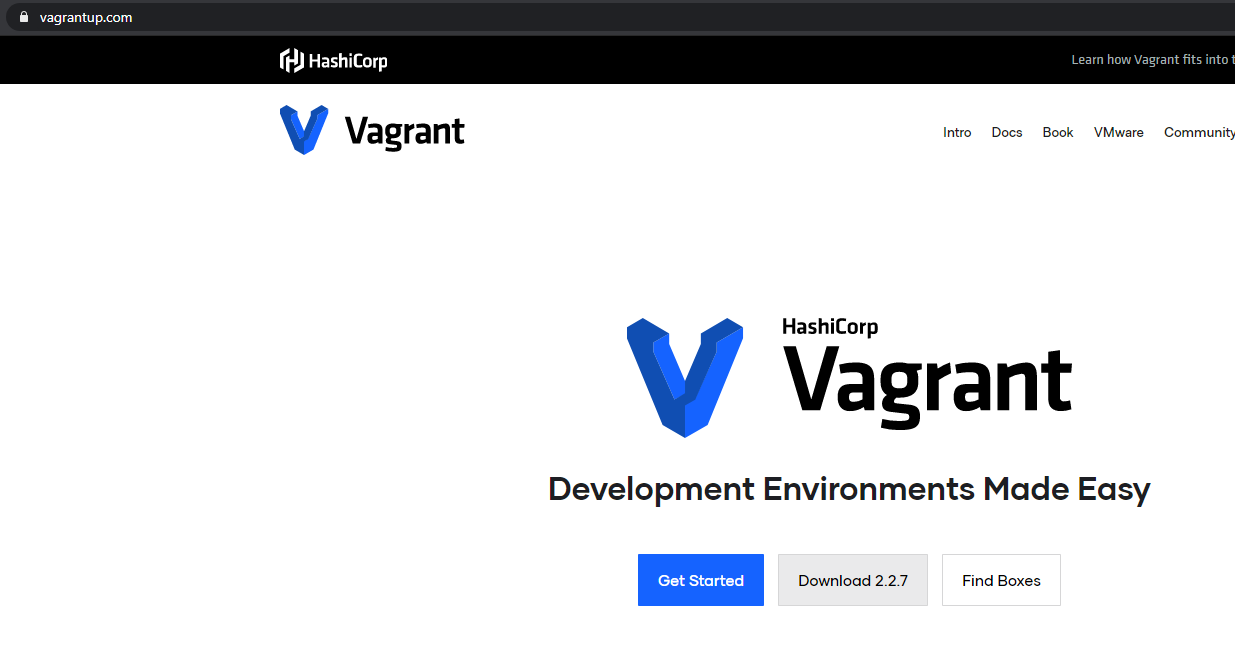
\includegraphics[scale=0.9]{img/install/vagrant0.png}
        \caption{Sitio web oficial de vagrant, sección de descarga}
        \label{fig:va0}
    \end{figure}
    
    Al momento de crear este documento Vagrant se encuentra en la versión 2.2.7. Durante el desarrollo de este proyecto el autor tuvo la posibilidad de realizar diferentes charlas en varios meetups del país: 
    
    \begin{itemize}
        \item Manizales Tech Talks
        \item Bucaramanga Js
        \item Pereira Tech Talks
    \end{itemize}
    
    Los slides de esta presentación puede ser encontradas en el sitio web  \url{https://slides.com/c1b3r/vagrant}.
    
    Es necesario, como se mencionó previamente, instalar vagrant con permisos de administrador; de la misma manera se sigue el setup wizard de Vagrant haciendo click en el boton \textbf{next}.
    \begin{center}
      \begin{figure}[H]
        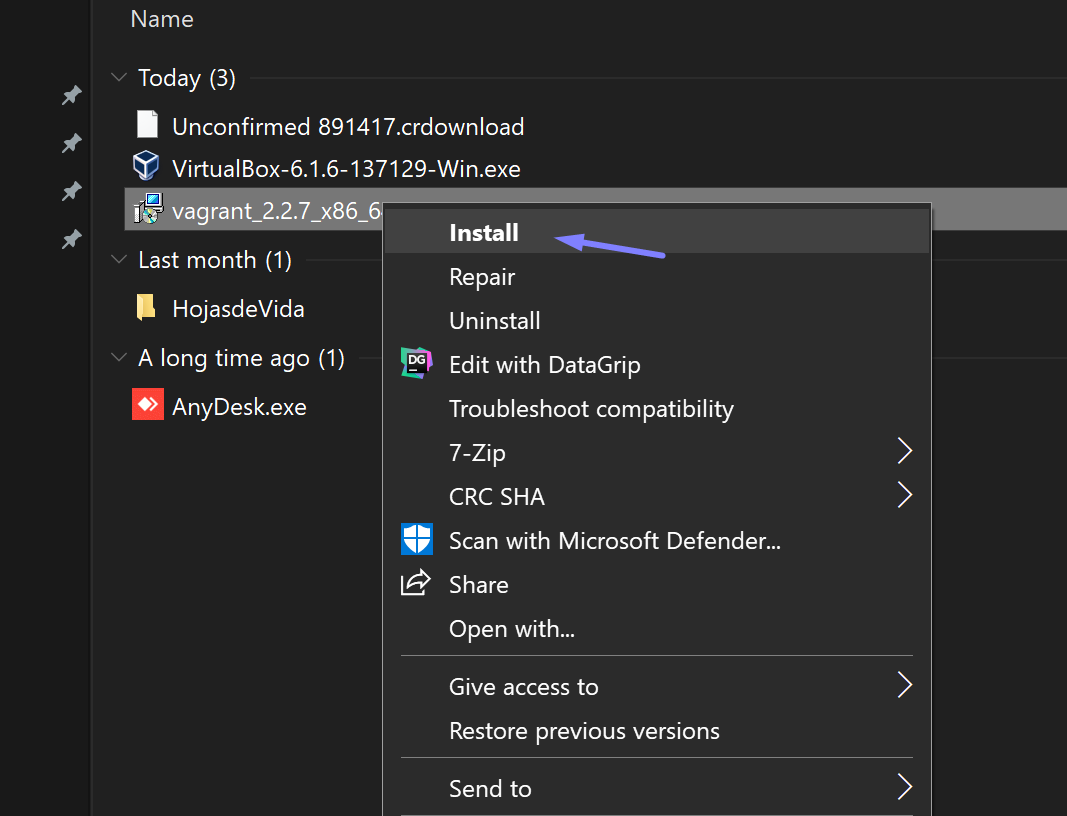
\includegraphics[scale=0.9]{img/install/vagrant1.png}
        \caption{Instalador de Vagrant, setup wizard.}
        \label{fig:va1}
    \end{figure}
    
     \begin{figure}[H]
        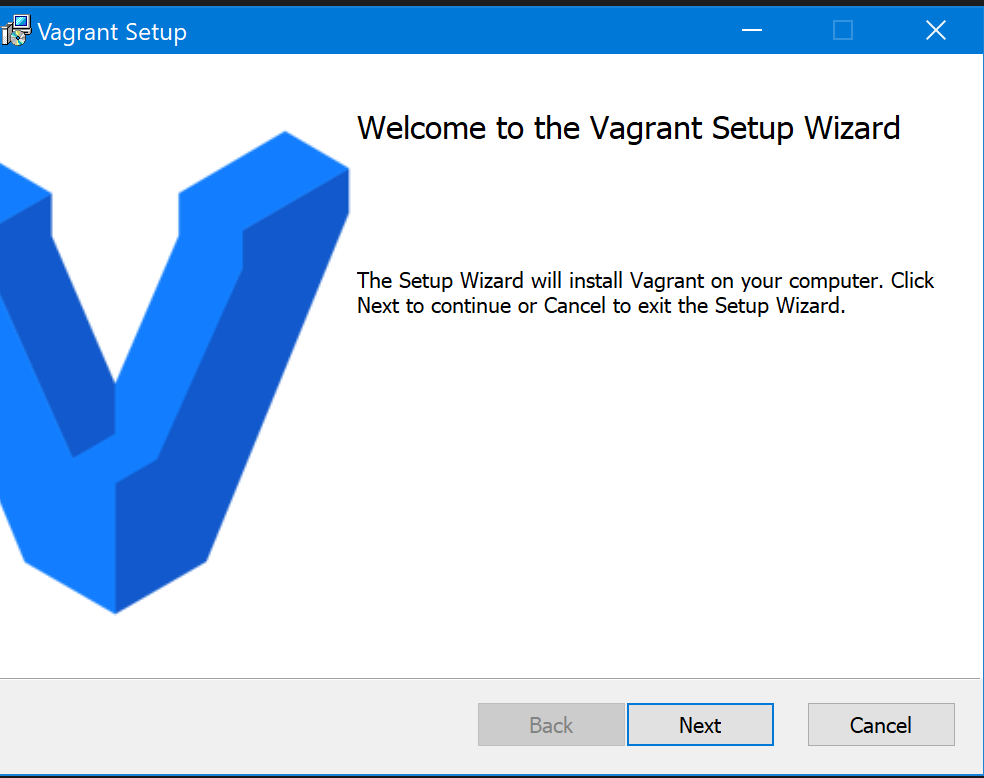
\includegraphics[scale=0.9]{img/install/vagrant2.png}
        \caption{Setup Wizard de Vagrant. }
        \label{fig:va2}
    \end{figure}     
    \end{center}
 
    \begin{center}
    \begin{figure}[H]
        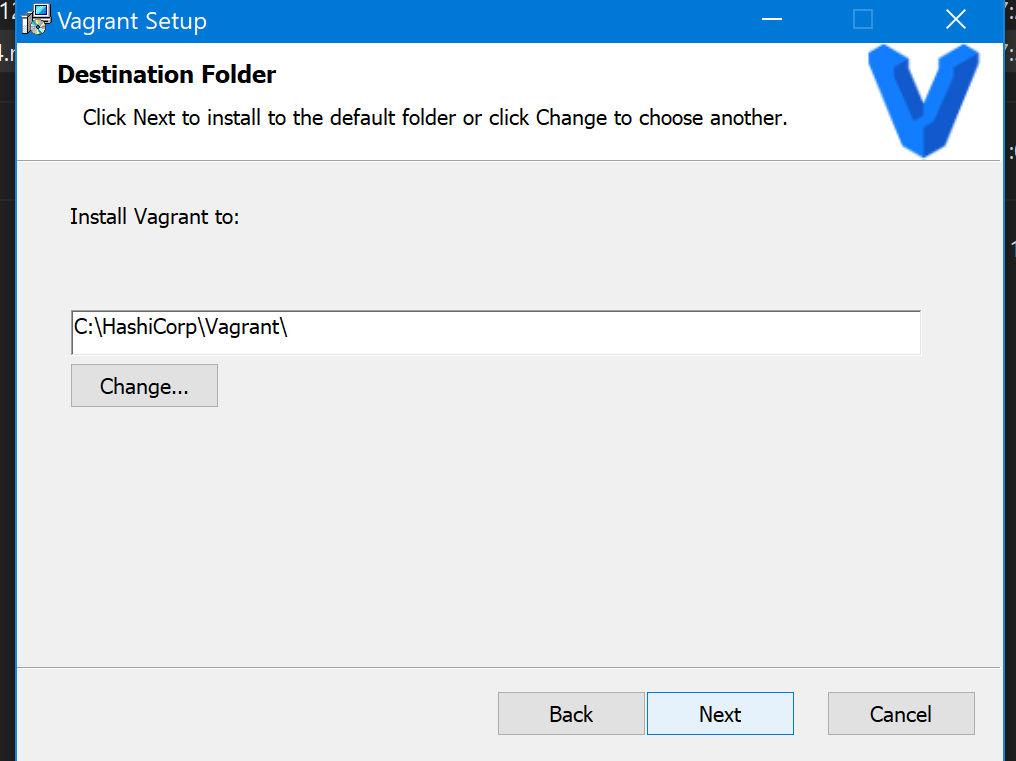
\includegraphics[scale=1.0]{img/install/vagrant3.png}
        \caption{Selección de ubicación para instalar Vagrant. La recomendación oficial es dejar en la ruta por defecto, ya que de esta forma no habrá conflicto para definirlo dentro de las variables de entorno (la definición dentro de las variables de entorno es realizado por Vagrant de manera automática).}
        \label{fig:va3}
    \end{figure}
    

     \begin{figure}[H]
        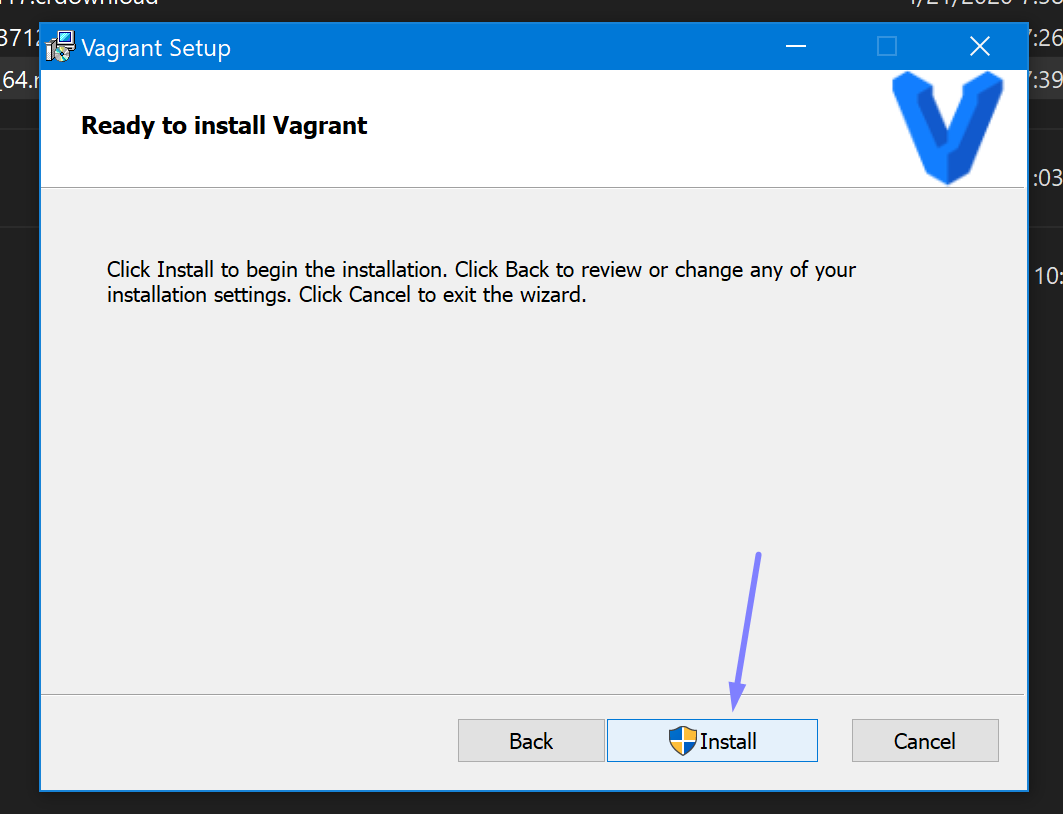
\includegraphics[scale=0.9]{img/install/vagrant4.png}
        \caption{Paso de confirmación para el install wizard}
        \label{fig:va4}
    \end{figure}
    
        \begin{figure}[H]
        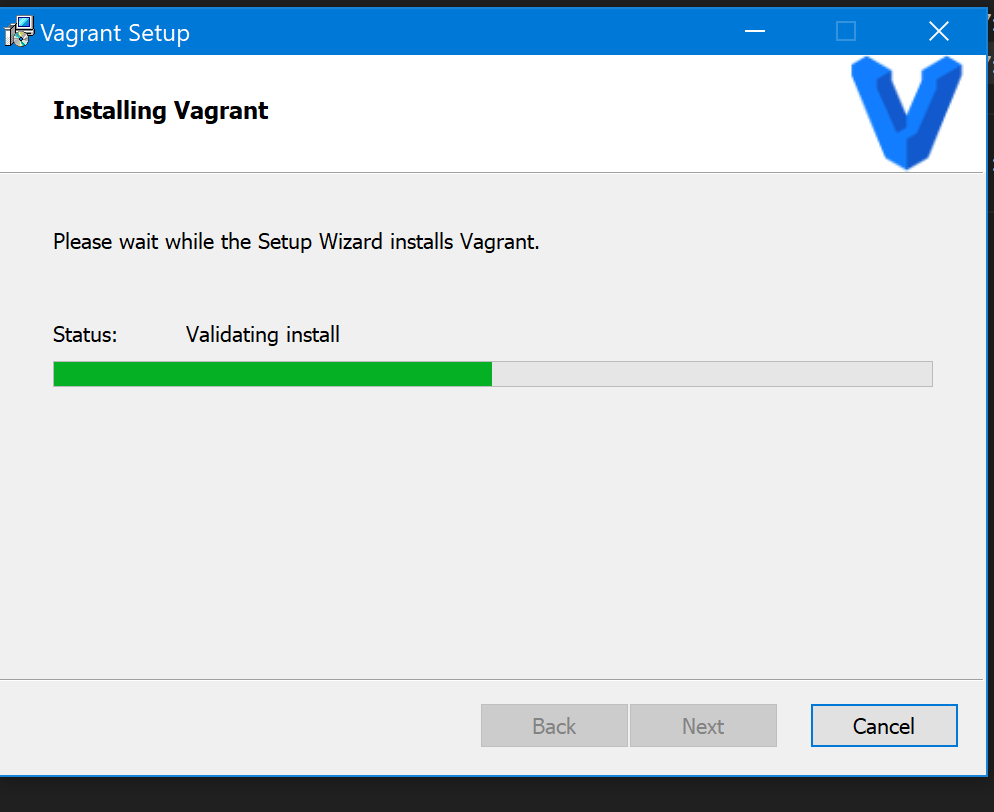
\includegraphics[scale=0.9]{img/install/vagrant5.png}
        \caption{Instalación de Vagrant en proceso.}
        \label{fig:va5}
    \end{figure}
    \end{center}
   
    Al momento de que el procedimiento guiado de instalación ha terminado, se debe abrir una consola de powershell o cmd para buscar que el comando está correctamente instalado y dentro de las variables de entorno.
    \begin{center}
    \begin{figure}[H]
        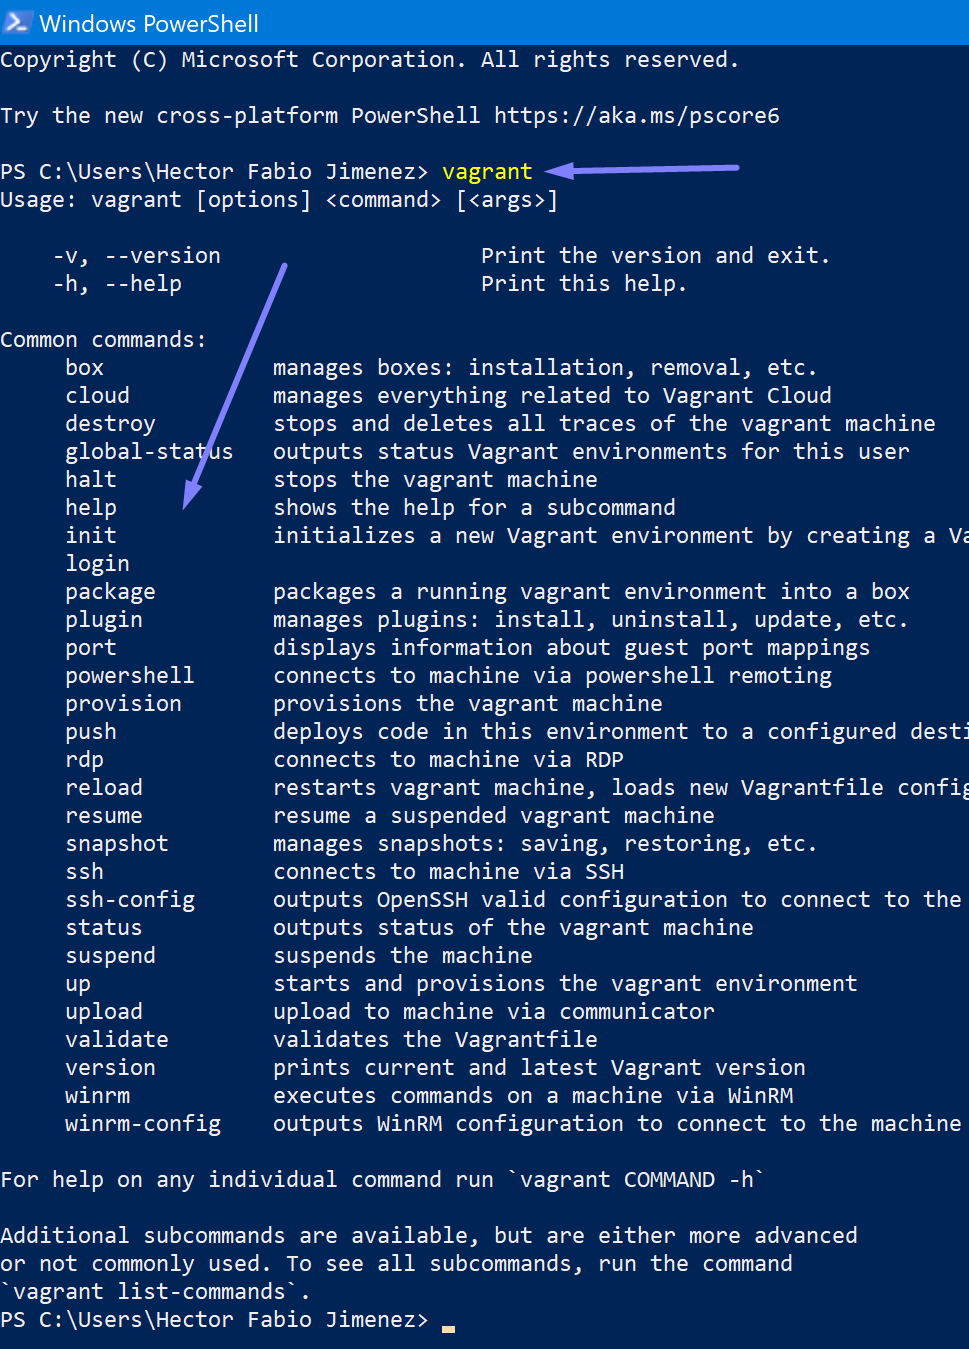
\includegraphics[scale=1.0]{img/install/vagrant6.png}
        \caption{Opciones disponibles de Vagrant en la línea de comandos.}
        \label{fig:va6}
    \end{figure}
    \end{center}
    
    \subsection{Pruebas de Aprovisionamiento Vagrant Boxes}
    Según el sitio web de Redhat Inc \cite{provisioning}, la etapa de aprovisionamiento se define como el conjunto de pasos requeridos para administrar el acceso a los datos y recursos, y de cómo es posible hacerlos disponibles a los usuarios y sistemas\cite{provisioning}. Microsoft y Vmware, por otro lado, en el contexto de las máquinas virtuales, indican que el aprovisionamiento son los diferentes mecanismos con las cuales se crean las máquinas virtuales \cite{provisioning2}\cite{provisioning3}.
    
    Al cumplir con los prerrequisitos de instalación de Vagrant y VirtualBox en el computador, es hora de proceder a correr un ejemplo muy básico donde se puede observar que el aprovisionamiento funciona adecuadamente entre Vagrant(\textit{ automatización descriptiva}) y VirtualBox(\textit{ hypervisor}).
    
    Esta prueba consiste en lanzar una máquina virtual utilizando ambas herramientas. Para realizarlo Vagrant solo necesita tener la instancia del archivo de configuración, este es llamado (\textbf{“Vagrantfile”}), su función primaria es describir el tipo de máquina requerida por proyecto y la definición de como aprovisiona la(s) máquina(s) virtuales. Este archivo es llamado así debido a que es el nombre literal del archivo que Vagrant va a intentar leer al momento de ejecutar el comando \textbf{\texttt{vagrant up}}. 
    Es necesario mencionar que Vagrant corre un solo archivo de configuración por proyecto, además este tendrá que ser versionado utilizando una herramienta como  \textit{Git}, de esta manera, un nuevo desarrollador que se integre al equipo simplemente tendrá que clonar el repositorio del proyecto y ejecutar \texttt{vagrant up} para tener el entorno de desarrollo montado y funcionando en cuestión de minutos. Por defecto, Vagrant utiliza VirtualBox como motor de máquinas virtuales o \textbf{provider}, aunque existe la opción de utilizar otros providers como VMWare Workstation (Windows) o VMWare Fusion (MacOS X) con un plugin de pago, AWS EC2 Web Services, Compute Engine de Google Cloud Platform.
    
    La sintaxis de los archivos de Vagrant utilizan Ruby, pero el conocimiento del lenguaje de programación no es necesario para hacer las modificaciones, dado que este trata la descripción de los recursos de una manera simple y concisa. 
    
    En los ejemplos de las Figuras  Figura.\ref{fig:vagrantfile1},  Figura.\ref{fig:vafile2} se puede observar claramente la descripción de hardware.
    
    El flujo de trabajo de vagrant está resumido en la figura Figura.\ref{fig:flow}, de la que se pueden resaltar los siguientes pasos: 
    \begin{enumerate}
        \item El desarrollador posee el archivo descriptivo \textbf{“Vagrantfile”} y ejecuta el comando \textbf{\texttt{vagrant up}}
        \item Vagrant, con su analizador léxico validará las descripciones de VirtualBox. También revisa si es necesario ejecutar algún provisioner\footnote{Los provisioners son opcionales, pero son de un uso común en la creación de entorno y despliegues de máquinas virtuales} como un script de bash, ansible, puppet entre otros; si no, este creará todo lo necesario con el hypervisor.
        \item La máquina virtual estará disponible para el desarrollo.
        \item Mediante ssh el desarrollador tendrá acceso a todo el entorno.
    \end{enumerate}
    $$\\$$
    \begin{figure}[H]
        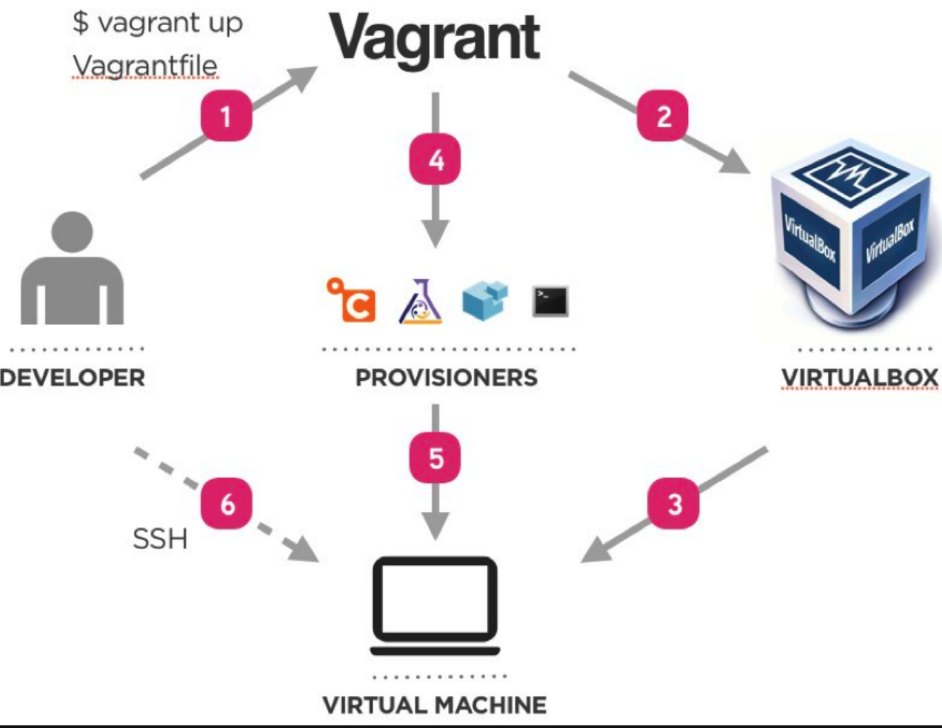
\includegraphics[scale=1.2]{img/install/vagrantworflow.png}
        \caption{Flujo de Trabajo de Vagrant, Etapas.}
        \label{fig:flow}
    \end{figure}
    
    \begin{figure}[H]
        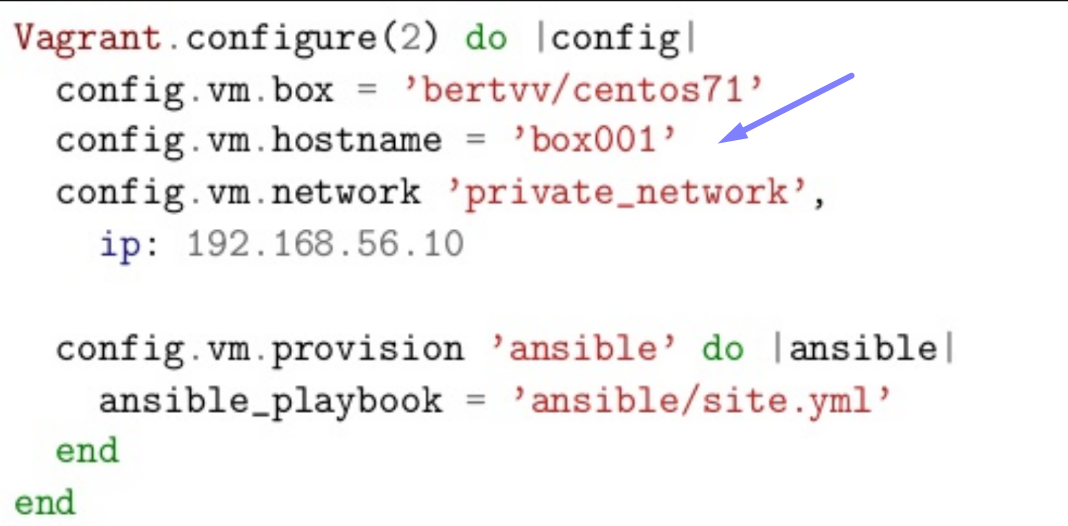
\includegraphics[scale=1.0]{img/install/vagrantfile.png}
        \caption{Ejemplo de Vagrantfile, versión 1. }
        \label{fig:vagrantfile1}
    \end{figure}
    
    \begin{figure}[H]
        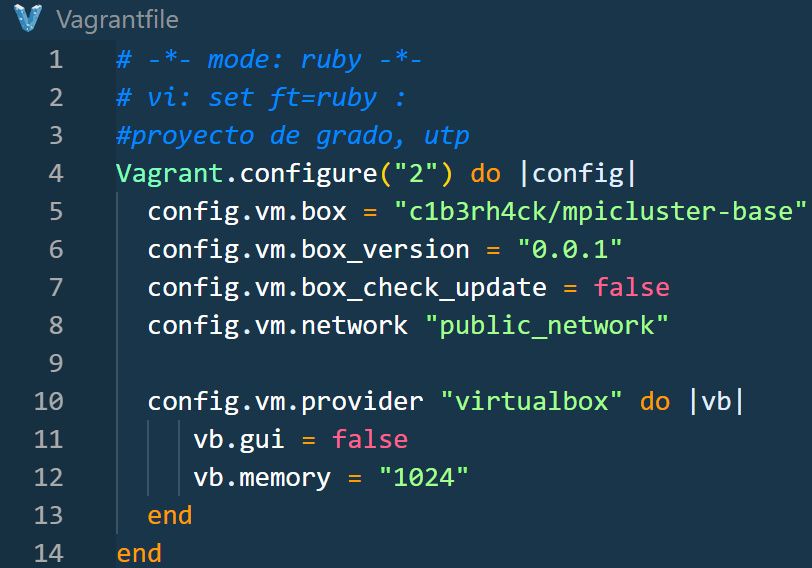
\includegraphics[scale=1.2]{img/provision/vagrantbox.png}
        \caption{Ejemplo de Vagrantfile, versión 2. }
        \label{fig:vafile2}
    \end{figure}
    
    
    \begin{figure}[H]
        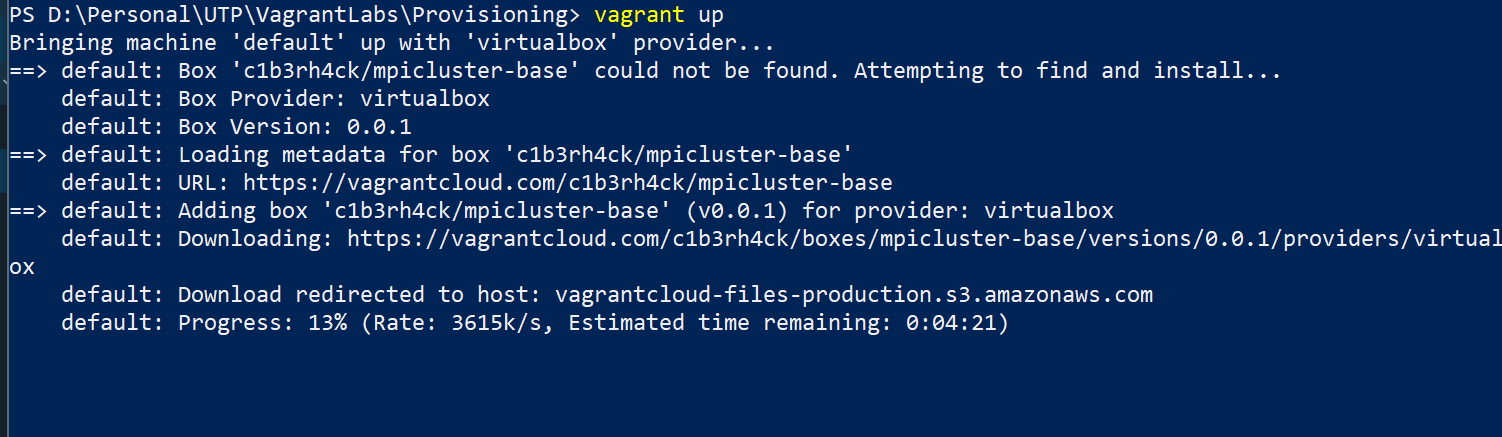
\includegraphics[scale=0.7]{img/provision/vagrantbox2.png}
        \caption{resultado de importación y creación de vagrant up.}
        \label{fig:va6}
    \end{figure}
    
    \begin{figure}[H]
        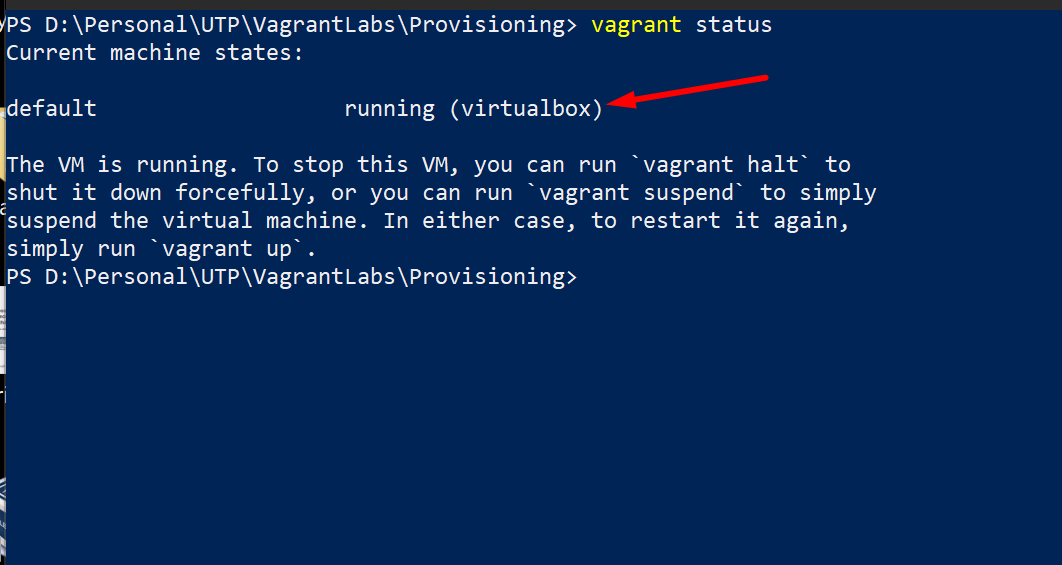
\includegraphics[scale=1]{img/provision/running.png}
        \caption{Aprovisionamiento Exitoso, Estado de la máquina virtual.}
        \label{fig:va6}
    \end{figure}
    \begin{center}
    \begin{figure}[H]
        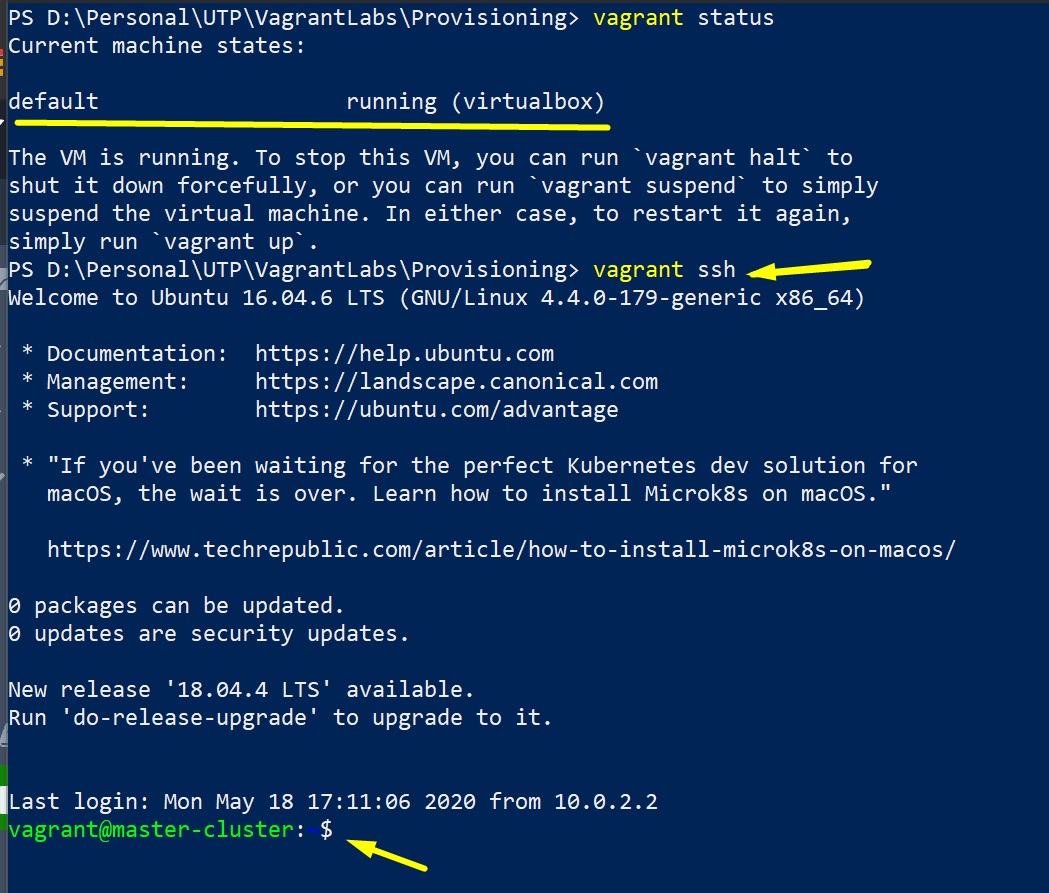
\includegraphics[scale=1]{img/provision/running2.png}
        \caption{Conexión exitosa a la máquina virtual aprovisionada, \textbf{\texttt{vagrant ssh}}.}
        \label{fig:va6}
    \end{figure}
    \end{center}
    \subsection{Pruebas de Networking y Direccionamiento}
    Oracle VM VirtualBox provee hasta 8 tarjetas virtuales Ethernet PCI para cada máquina virtual. Para cada tarjeta, se puede seleccionar individualmente lo siguiente: 
    \begin{itemize}
        \item Hardware que será virtualizado.
        \item Modo de Virtualización que la tarjeta usará en su modo de operación con respecto al hardware de red en la máquina host entre los modos Nat, Bridge, Red Interna.
    \end{itemize}
    
    Siempre en la interfaz gráfica de VirtualBox se podrá configurar hasta 4 tarjetas tal cual como se muestra en la Figura.\ref{fig:net1}, las otras 4 tarjetas de red pueden ser configuradas utilizando las opciones de línea de comandos provista por VirtualBox \textit{\texttt{VBoxManage modifyvm}}\cite{vbnet1}.
    
    \begin{figure}[H]
        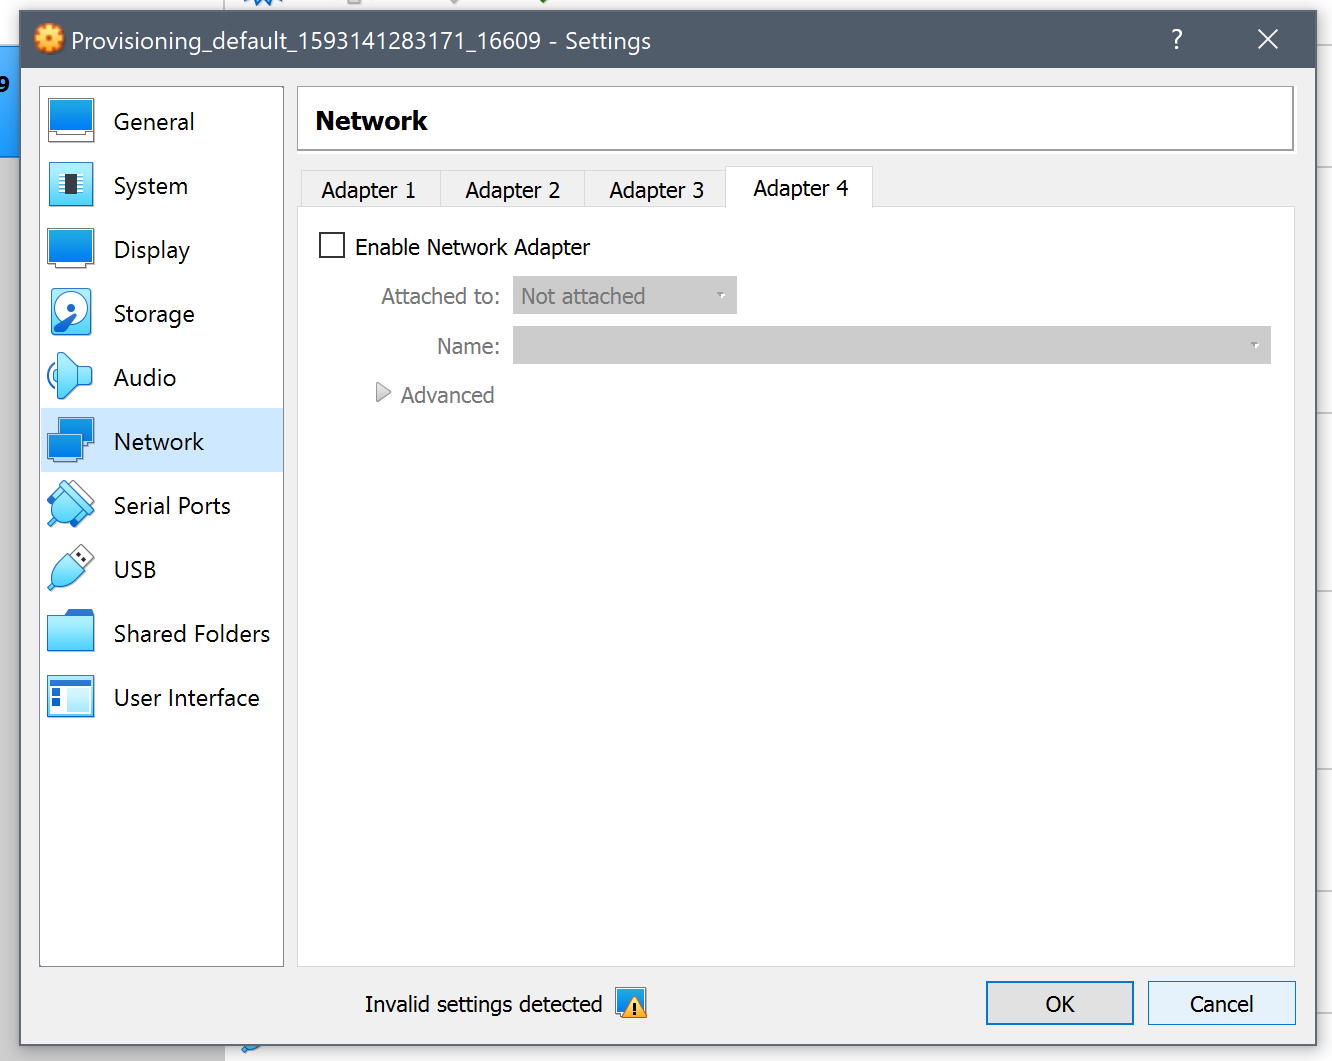
\includegraphics[scale=0.8]{img/networking/networking1.png}
        \caption{Sección de red, máquina virtual aprovisionada.}
        \label{fig:net1}
    \end{figure}
    Como se mencionó previamente, los modos de virtualización de las tarjetas de red de VirtualBox definen la visibilidad en un segmento de red y el alcance de las máquinas virtuales, también las capacidades que tendrá la máquina virtual a nivel de networking. A continuación se presenta un resumen de los modos, donde se denota si las máquinas virtuales alcanzan el equipo host, o a varias máquinas virtuales entre sí o con una red especifica.
    
    \begin{figure}[H]
        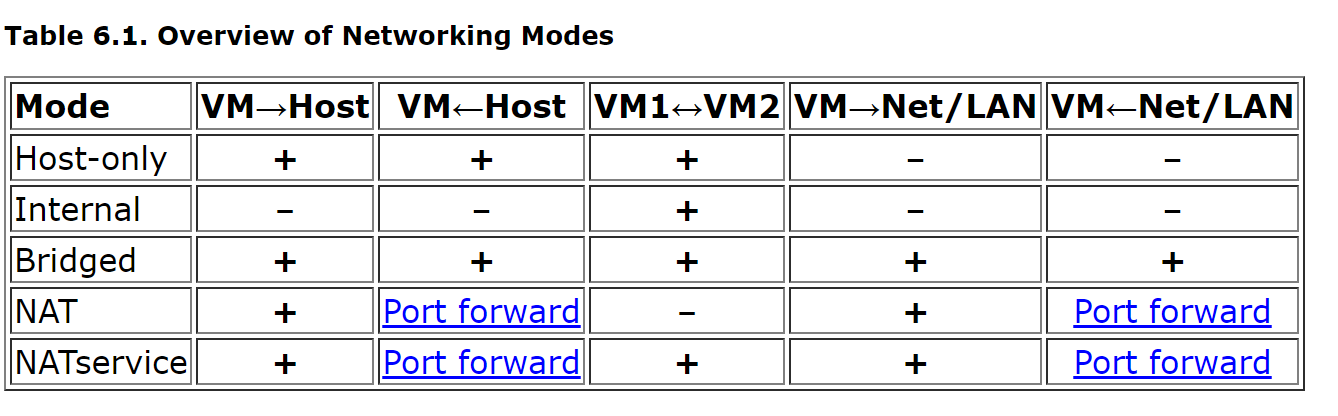
\includegraphics[scale=0.8]{img/networking/networking3.png}
        \caption{Conexión a la máquina virtual aprovisionada, \textbf{\texttt{vagrant ssh}}.}
        \label{fig:net33}
    \end{figure}
    
    Por ejemplo, si se mira el modo Host-Only de la Figura.\ref{fig:net33} se puede observar: 
    \begin{itemize}
        \item La conexión entre la máquina virtual y el Sistema operativo se puede establecer en ambos sentidos, según las flechas indicativas. 
        \item La conexión entre múltiples máquinas virtuales se puede realizar en ambos sentidos.
    \end{itemize}
    
    \begin{center}
         \begin{figure}[H]
            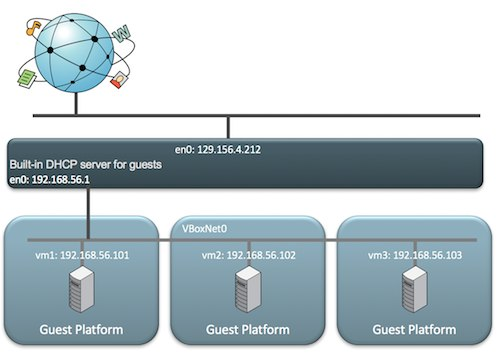
\includegraphics[scale=1.4]{img/networking/host_only.jpg}
            \caption{Conexión usando el modo Host Only, Implementación del Cluster MPI, cada máquina virtual Guest queda en el mismo segmento de red permitiendo comunicación bidireccional.}
            \label{fig:net21}
        \end{figure}
    \end{center}
   
   Además de los diferentes modos provistos por VirtualBox, este también provee un administrador de redes, donde se permite administrar los segmentos y las redes creadas. En la Figura.\ref{fig:net2} se observa que cada vez que se crea una red LAN utilizando VirtualBox Network Manager este crea a su vez los dispositivos de red virtuales en el sistema operativo host. Si estos dispositivos no se encuentran creados al momento de aprovisionar el clúster, Vagrant realiza su creación de manera automática.
    
    \begin{figure}[H]
        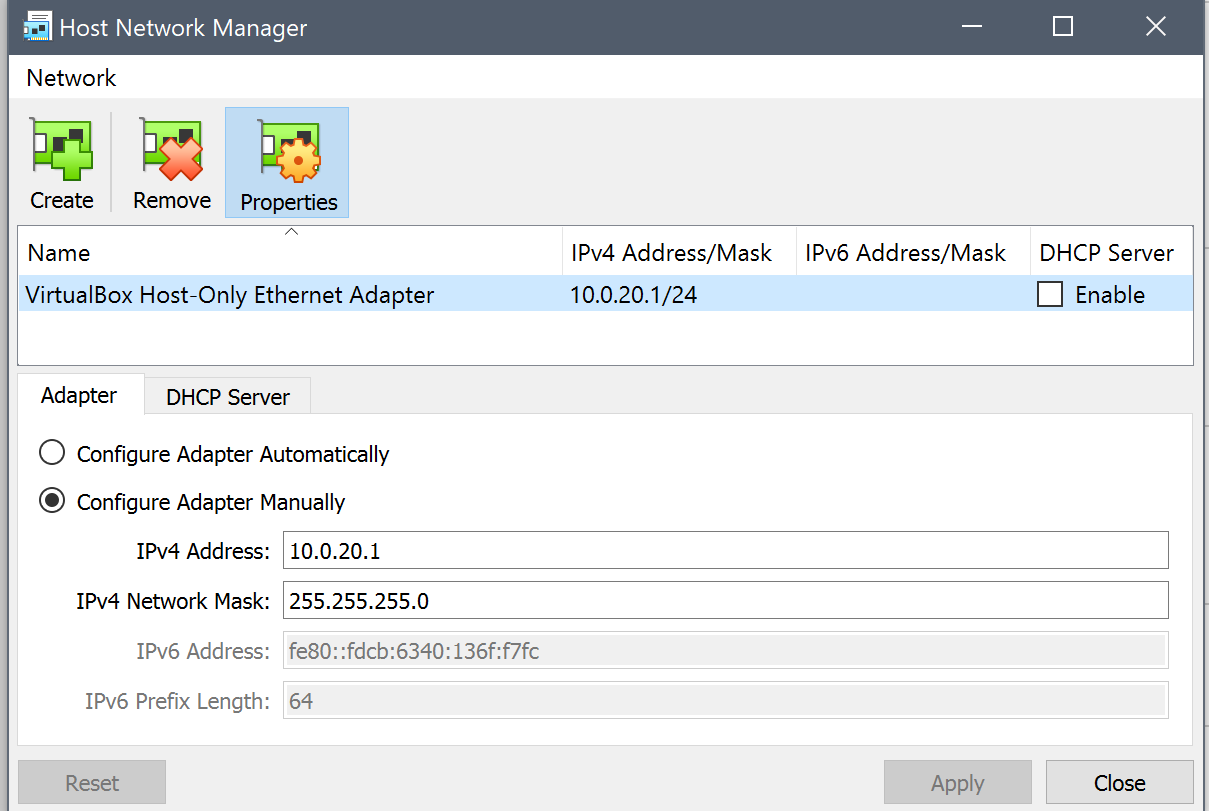
\includegraphics[scale=1]{img/networking/networking2.png}
        \caption{Conexión a la máquina virtual aprovisionada, \textbf{\texttt{vagrant ssh}}.}
        \label{fig:net2}
    \end{figure}
    \subsubsection{Opciones de Configuración Programáticas Vagrant}
    Vagrant a través de su declaración programática expone opciones de alto nivel para manipular las configuraciones de las tarjetas de red y las redes creadas por VirtualBox, entre ellas: 
    \begin{itemize}
        \item Configuraciones de PortForwading.
        \item Configuraciones de múltiples segmentos de red por tarjeta virtual.
        \item Creación de redes privadas.
    \end{itemize}
    
    
    \begin{figure}[H]
        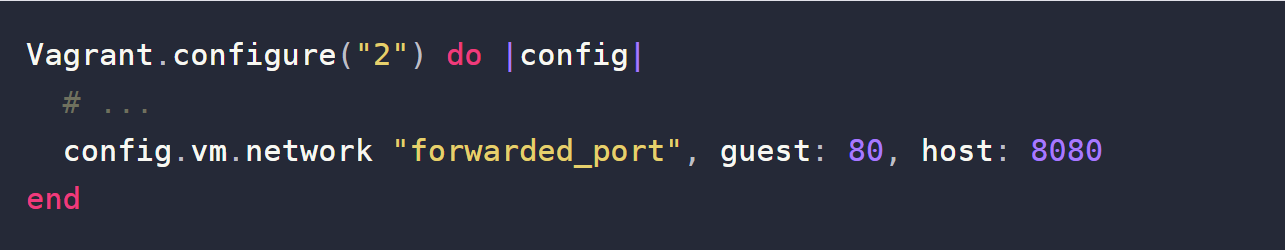
\includegraphics[scale=0.8]{img/vagrantport/vagrantportforwading.png}
        \caption{Port Forwarding .}
        \label{fig:forward1}
    \end{figure}
    
    En la Figura.\ref{fig:forward1} Se puede observar como se realiza de manera declarativa la exposición del puerto \textbf{80} en la máquina virtual y que se reflejará en el puerto \textbf{8080} en la máquina host.
    
    También declarativamente se puede establecer diferentes puertos, además del tipo de protocolo como se observa en la Figura.\ref{fig:forward2}
    
    \begin{figure}[H]
        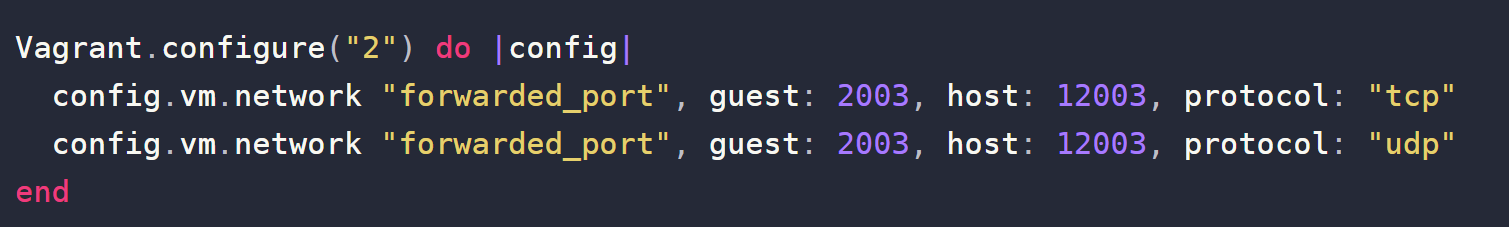
\includegraphics[scale=0.7]{img/vagrantport/portforwaded2.png}
        \caption{Multiple Port Forwarding, con puertos diferentes en máquina host e invitado, especificando protocolo.}
        \label{fig:forward2}
    \end{figure}
    Vagrant también permite especificar los tipos de redes, como por ejemplo las redes privadas que le permiten acceder a su máquina virtual por alguna dirección que no sea públicamente accesible desde Internet o en la misma LAN de la máquina host. En general, esto significa que la  máquina virtual obtiene una dirección en el espacio de direcciones privadas.
    \begin{figure}[H]
        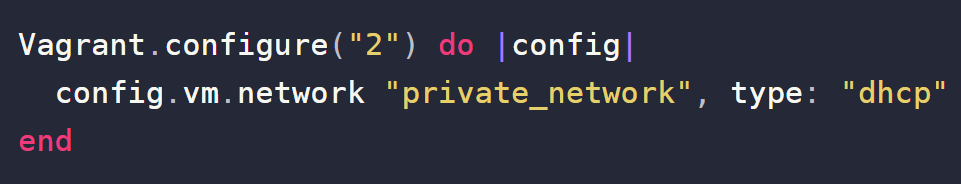
\includegraphics[scale=1.2]{img/vagrantport/privadadhcp.png}
        \caption{Declaración de red privada, asignación de IP por dhcp.}
        \label{fig:forward2}
    \end{figure}
    
    \begin{figure}[H]
        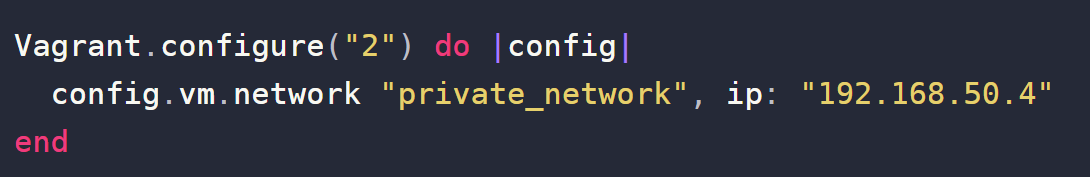
\includegraphics[scale=1.1]{img/vagrantport/privadastatic.png}
        \caption{Declaración de red privada, asignación de dirección ipv4 estática.}
        \label{fig:forward2}
    \end{figure}
    
    \subsection{Aprovisionamiento de Múltiples Maquinas Virtuales}
    Vagrant permite realizar la instanciación de la cantidad que se desee de máquinas virtuales en un mismo Vagrantfile. Nótese cómo en la Figura.\ref{fig:provision1} la definición quiere crear dos máquinas virtuales al mismo tiempo: una con el nombre de \textbf{web} y otra con el nombre \textbf{db}, la primera basada en una imagen de \textit{apache} y la segunda de \textit{mysql}.
    \begin{figure}[H]
        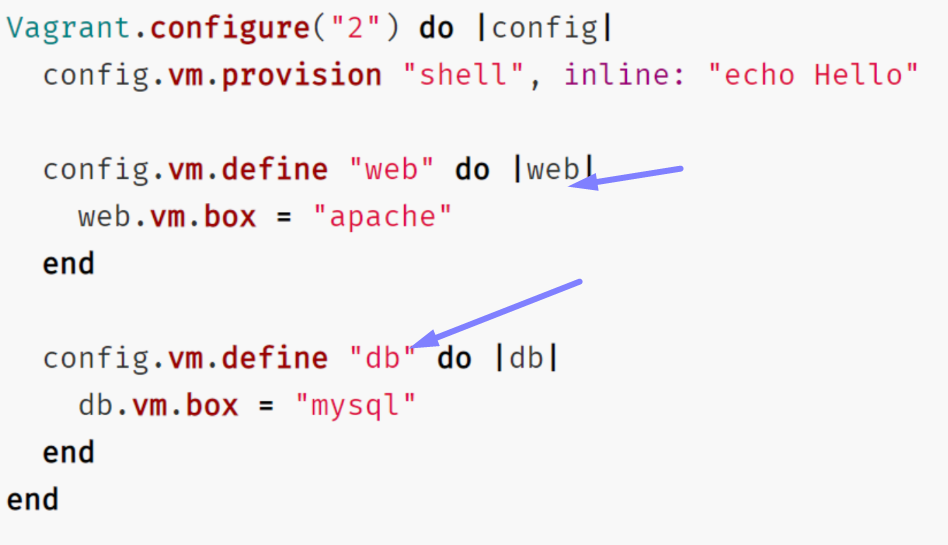
\includegraphics[scale=0.9]{img/cluster/multi1.png}
        \caption{Defunción de Múltiples máquinas virtuales, \textbf{\texttt{vagrant ssh}}.}
        \label{fig:provision1}
    \end{figure}
    
    Por otra parte, en la definición de las máquinas virtuales la herramienta permite realizar iteraciones como se muestra en la Figura.\ref{fig:provision2}, donde se crean tres máquinas virtuales y se da el nombre de \textbf{\textit{node-\#i}}, De esta misma manera se realiza la configuración de los nodos del cluster MPI.
    
    \begin{figure}[H]
        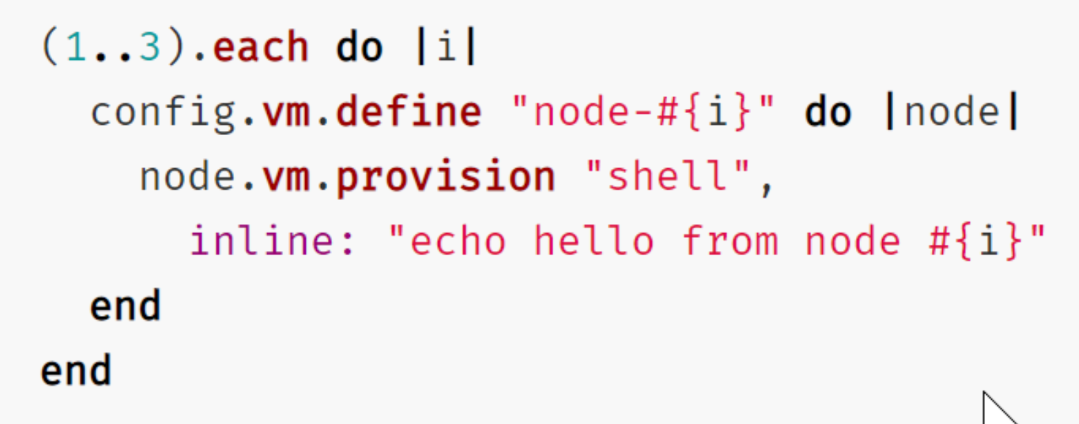
\includegraphics[scale=0.8]{img/cluster/multi2.png}
        \caption{Conexión a la máquina virtual aprovisionada, \textbf{\texttt{vagrant ssh}}.}
        \label{fig:provision2}
    \end{figure}
    
    \subsection{Sistema de Archivos Compartido clúster MPI}
    El protocolo NFS ha existido durante casi mas de 20 años desde su primer RFC publico \textit{rfc1094} \cite{nfsv1}, es el protocolo de intercambio de archivos de red de facto para sistemas operativos Unix y Gnu/Linux. El protocolo NFS se encuentra en su cuarta versión y esta a cargo de investigadores de todo el mundo, con desarrolladores y científicos de todo el mundo. El protocolo NFS proporciona acceso remoto y transparente a archivos y recursos compartidos en red, este está diseñado para ser portable y multiplataforma además de ser soportado en diferentes tipos de máquinas, sistemas operativos, arquitecturas de redes y protocolos de transporte. 
    Su portabilidad y funcionamiento se logra mediante el uso de primitivas RPC integradas junto con la representación de datos externos (XDR, eXternal Data Representation). 
    
    En la actualidad la versión estable de este protocolo es la \textbf{NFSv4},  con importantes mejoras como el soporte para manejar sistemas de archivos de 64bits, escritura de archivos asíncronas, funcionamiento a través de firewalls y soporte  para configuraciones de listas de control de acceso \textbf{NFSv4}. El clúster MPI requiere de un sistema de archivos compartido entre el nodo maestro y los nodos esclavos para poder compartir el binario que se ejecutará como parte de las llamadas MPI. 
    
    \begin{figure}[H]
    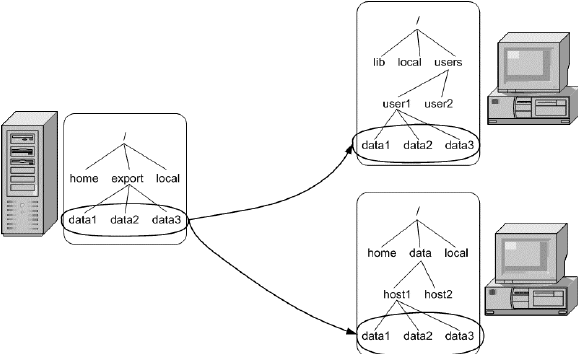
\includegraphics[scale=0.7]{img/nfs/nfs.png}
    \caption{Funcionamiento de NFS.}
        \label{fig:nfs1}
    \end{figure}
    El protocolo NFS trabaja como un servicio sobre un sistema de archivos real, trabaja con archivos en vez de trabajar con bloques, a manera de un sistema de archivos distribuido. En la Figura.\ref{fig:nfs1} se observa claramente como en esta arquitectura cliente servidor, el servidor equipo de la izquierda exporta un directorio de nombre \texttt{\textit{\//export}}, debajo de este hay varios archivos (\texttt{\textit{data1,data2,data3}}). Al lado derecho se puede observar dos equipos que cumplen la función de cliente, estos mediante un cliente nfs montan el recurso compartido por el servidor; cuando el cliente termina de negociar los diferentes parámetros permite que los clientes tengan acceso a los mismos datos del servidor. Notese que cada cliente puede elegir la ubicación en la que desea montar el sistema de archivos, en el caso del cliente de la parte superior su punto de montaje es  \texttt{\textit{\//users/user1/}} y el otro \texttt{\textit{\//data/host1/}}.
    
    \begin{figure}[H]
    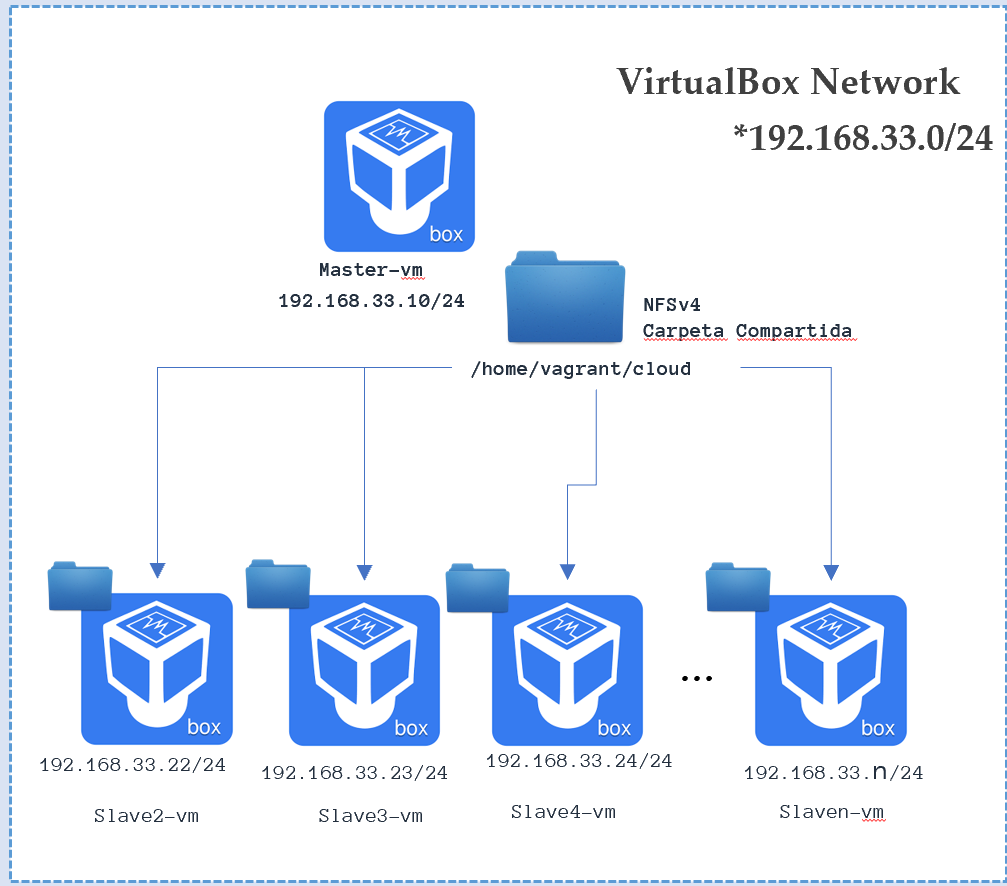
\includegraphics[scale=1]{img/nfs/nfs2.png}
    \caption{Funcionamiento de NFS, ejemplo basico NFSv3.}
        \label{fig:net3}
    \end{figure}
    
    Para el desarrollo de este trabajo, como se menciona previamente es necesario realizar el montaje de un sistema de archivos compartido, este permitirá que almacenemos los binarios de los programas con las sentencias de MPI. Se ha elegido la ubicación \texttt{\textit{\//home/vagrant/\textbf{cloud}}} para la instalación del sistema de archivos compartido, esto se hace en un sistema operativo Ubuntu 16.04, tal cual como se muestra en los comandos de la Figura.\ref{fig:nfsserver}
      \begin{figure}[H]
            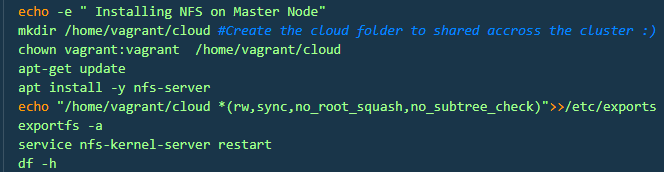
\includegraphics[scale=1.8]{img/nfs/installnfs.png}
            \caption{Instalación Servidor NFSv4.}
            \label{fig:nfsserver}
    \end{figure}
    
    Se observa como en la máquina que actúa como servidor se instala el paquete \texttt{nfs-server} al cual se le pasan todas las opciones para el recurso compartido, en este caso : 
    \begin{itemize}
        \item rw : Permisos para lectura y escritura en el folder.
        \item sync : Permisos para lectura y escritura en el folder.
        \item no\_root\_squash : No se desea que el usuario root del equipo que monta el sistema de ficheros equivalga al root del sistema que lo exporta.
        \item no\_subtree\_check : Mejora el performance, deshabilitando la revisión del arbol del sistema de archivos en todo los clientes y servidor.
    \end{itemize}
    $\\$
    $echo "/home/vagrant/cloud *(rw,sync,no\_root\_squash,no\_subtree\_check)">>/etc/exports$
    
    
    En todos los clientes, se realiza la instalación del paquete \texttt{nfs-common} con el fin de poder montar el sistema de archivo exportado por el servidor.
    
    \begin{figure}[H]
            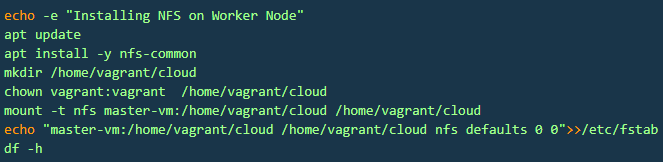
\includegraphics[scale=1.8]{img/nfs/installnfscliente.png}
            \caption{Configuración NFSv4, Clientes del Cluster.}
            \label{fig:cGetlus0}
    \end{figure}
    
    Para los clientes basta con agregar una línea donde se indica al cliente que monte todos los archivos compartidos por el servidor en la carpeta local con las configuraciones por defecto.
    \newpage    
    \subsection{Configuraciones de Seguridad}
    Las configuraciones de seguridad realizadas para este proyecto son técnicas y métodos ampliamente difundidos por los desarrolladores y administradores de las distribuciones de sistemas operativos GNU/Linux\cite{LINUXHARDENING}\cite{LINUXHARDENING2}\cite{LINUXHARDENING3}, entre ellas las siguientes:
    \begin{itemize}
        \item Documentar la información de las máquinas virtuales en el clúster, recolectando datos como el nombre de la máquina, dirección IP, dirección MAC y el número de asset (recurso).
        
        \item Al tratarse de máquinas virtuales, es necesario asegurar que el sistema de arranque no sea modificado por personas externas al hypervisor.
        
        \item Las máquinas virtuales deben contar con las últimas actualizaciones que el sistema operativo tenga disponibles, esto se logra mediante la ejecución, en el caso de la distribución Ubuntu, del comando \textit{ \texttt{apt-get update} }.
        
        \item Deshabilitar servicios innecesarios del sistema, que vienen por defecto.
        
        \textit Realizar un listado de usuarios permitidos para la ejecución de programas MPI en cada uno de los nodos del clúster y se configuran las llaves de seguridad comunes para alcanzar el nodo maestro.
        
    \end{itemize}
    
    \subsection{Pruebas de clúster MPI Multimaquina}
    Finalmente después de haber realizado la comprensión total de los diferentes elementos que se deben configurar a continuación en la Figura.\ref{fig:clus0} se muestra una arquitectura de nuestro cluster  
    \begin{figure}[H]
            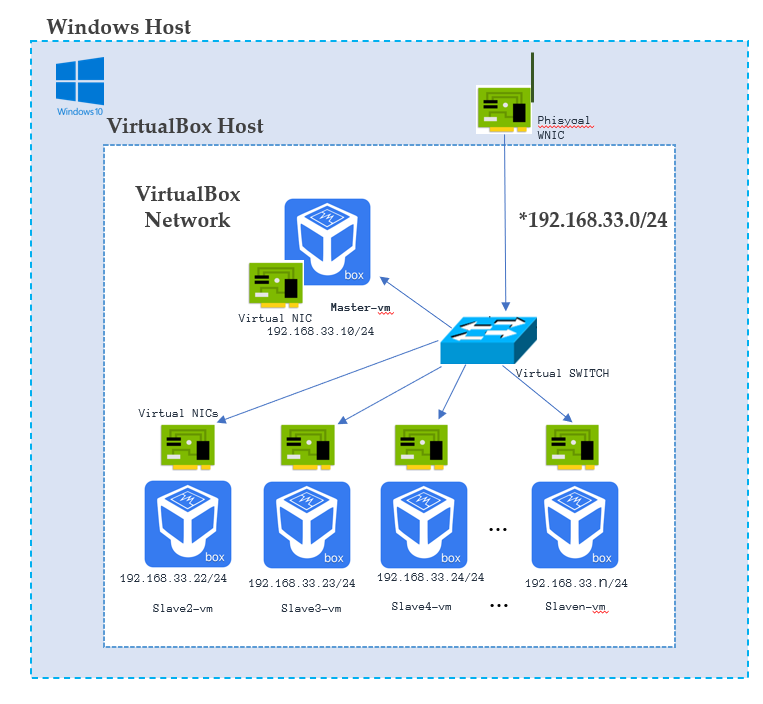
\includegraphics[scale=1.5]{img/cluster/cluster1.png}
            \caption{Arquitectura funcional cluster MPI, virtual switch .}
            \label{fig:clus0}
    \end{figure}
    Como se observa en la Figura.\ref{fig:clus0} tenemos una arquitectura compuesta por un nodo maestro de nombre \textbf{\texttt{Master-vm}} con dirección ipv4 192.168.33.10 perteneciente al segmento de red 192.168.33.0/24 en esta maquina virtual se instala el servidor de archivos NFSv4 (\textit{ver Figura.\ref{fig:nfsserver}, Figura.\ref{fig:net3}}), 
    
    \subsection{Ejecución sobre algoritmos clúster MPI}
    
    \clearpage
    
    \section{Resultados}
    

    \clearpage
    
    \section{Participantes}
    \begin{itemize}
        \item Hector Fabio Jimenez Saldarriaga, Estudiante de pregrado en Ingeniería De Sistema Y Computación: Planear, ejecutar, documentar y evaluar el proyecto.
        \item Ramiro Andrés Barrios Valencia, MSc. Ingeniería de Sistemas y Computación, Especialista en Electrónica Digital: Director y Asesor del proyecto.
    \end{itemize}
    
    \section{Recursos y Presupuesto}
    \subsection{Recursos Humanos}
    \begin{itemize}
        \item Director de proyecto.
    \end{itemize}
    
    \subsection{Recursos Físicos}
    \begin{itemize}
	    \item Laboratorio Sirius, CIDT. \\
	    Ingeniería de Sistemas. Universidad Tecnológica de Pereira. 
        \item Grupo de Investigación Sirius. \\
        Ingeniería de Sistemas y Computación. Universidad Tecnológica de Pereira.
        \item clúster Lovelace, Bloque L.
        \item Computador Tesista, Servidores Físicos a disposición tesista.
        \item Locaciones Grupo de Investigación Sirius. \par Ingeniería de Sistemas y Computación. Universidad Tecnológica de Pereira
        \item Biblioteca. Universidad Tecnológica de Pereira
	\end{itemize}
	
	A continuación un valor estimado para los recursos considerados en el proyecto:
	\begin{table}[t]
    \centering
    \begin{tabular}{}
    %table content
    \end{tabular}
    \caption{}
    \label{tab:label}
    \end{table}

	\begin{center}
    \begin{tabular}{|p{2.5cm}|p{3cm}|p{2cm}|p{2cm}|p{3cm}|}
    \hline
    \textbf{Recurso Humano} & \textbf{Costo(Peso Colombiano) / Hora } & \textbf{Número Horas} & \textbf{Total} & \textbf{Fuente Financiadora} \\
    \hline
    Investigador (Tesista   ) & 6.500 & 200 & 1.300.000 & Universidad \\
    \hline    \hline
    Director / Asesor & 38.000 & 80 & 3.040.000 & Universidad \\
    \hline
    \textbf{Compra o Alquiler de máquinaria y Equipos} & \textbf{Costo(Peso Colombiano) } & \textbf{Cantidad} & \textbf{Total} & \textbf{Fuente Financiadora} \\
    \hline
    Computador Thinkpad X1 6TH, procesador i7 8GEN, 1TB DD y 16GB RAM & 8.100.000 & 1 & 8.100.000 & Tesista  \\
    \hline

    \textbf{Fungibles} & \textbf{Costo(Peso Colombiano) } & \textbf{Cantidad} & \textbf{Total} & \textbf{Fuente Financiadora} \\
    \hline
    Papelería y otros & 50.000 &  & 50.000 & Tesista \\
    \hline
    Servicios públicos & 130.000 &  & 130.000 & Tesista  \\
    \hline
    \textbf{Costo Total del Proyecto} &  &  & 12.620.000 &  \\
    \hline
    \end{tabular}

    \end{center}\\
    
   
    
    \section{Cronograma}
    A continuación se describe un esquema de las actividades que se desarrollarán durante el proyecto, cada una consu respectiva duración:
    
    \begin{center}
    \begin{tabular}{|p{9.5cm}|p{0.4cm}|p{0.4cm}|p{0.4cm}|p{0.4cm}|p{0.4cm}|p{0.4cm}|}
    \hline
    \multicolumn{7}{|c|}{\textbf{Cronograma de Actividades}}\\
    \hline
    \textbf{Actividad / Tiempo(Meses)} & \textbf{1} & \textbf{2} & \textit{\textbf{3}} & \textbf{4} & \textbf{5} & \textbf{6} \\
    \hline
    Consultas e investigación sobre MPI, clúster y computación de alto rendimiento. & X &   &   &   &   &   \\
    \hline
    Investigación y Consulta de Infraestructura como Código, entendimiento del funcionamiento interno de Vagrant & X &   &   &   &   &   \\
    \hline
    Pruebas de aprovisionamiento automático de diferentes elementos de infraestructura con Vagrant & X &   &   &   &   &   \\
    \hline
    Implementación de algoritmos y scripts para la instalación de utilidades &  & X  &   &   &   &   \\
    \hline
    Pruebas de funcionamiento comunicación master-nodos &   &   & X &   &   &   \\
    \hline
    Ejecución de algoritmo en clúster &   &   &   & X &   &   \\
    \hline
    Elaboración de informe final &   &   &   &   & X &   \\
    \hline
    Entrega &   &   &   &   &   & X \\
    \hline
    \end{tabular}
    \end{center} \\
    
    \clearpage
    
    \section{Conclusiones}
    
    \clearpage
    
    \section{Bibliografía}
    
    \bibliographystyle{acm}
    \nocite{*}
    \bibliography{biblio}

\end{document}


 